% ==========================================================
% Computer Vision — Exam Summary
% Main sections follow the lecture sessions.
% ==========================================================

\documentclass[11pt,a4paper]{article}

% =======================
% Page + typography
% =======================
\usepackage[a4paper,margin=2.2cm]{geometry}
\usepackage[T1]{fontenc}
\usepackage[utf8]{inputenc}
\usepackage{lmodern}
\usepackage{microtype}
\usepackage{parskip}

% =======================
% Math
% =======================
\usepackage{amsmath,amssymb,amsfonts,mathtools}
\usepackage{bm}
\DeclareMathOperator*{\argmin}{argmin}
\DeclareMathOperator*{\argmax}{argmax}
\DeclareMathOperator{\tr}{tr}

\newcommand{\R}{\mathbb{R}}
\newcommand{\vct}[1]{\bm{#1}}
\newcommand{\mat}[1]{\mathbf{#1}}
\newcommand{\T}{^\mathsf{T}}
\newcommand{\inv}{^{-1}}
\newcommand{\norm}[1]{\left\lVert#1\right\rVert}

% =======================
% Figures, tables, lists
% =======================
\usepackage{graphicx}
\graphicspath{{figures/}}
\usepackage{subcaption}
\usepackage{booktabs}
\usepackage{siunitx}
\usepackage{enumitem}
\setlist[itemize]{topsep=2pt,itemsep=2pt,parsep=0pt,leftmargin=*}
\setlist[enumerate]{topsep=2pt,itemsep=2pt,parsep=0pt,leftmargin=*}

% Optional: for simple diagrams (enable if you use it)
\usepackage{tikz}
\usetikzlibrary{positioning}
\usetikzlibrary{arrows.meta}

% =======================
% Links + references
% =======================
\usepackage{xcolor}
\usepackage[hidelinks]{hyperref}
\usepackage[nameinlink,noabbrev]{cleveref}

% =======================
% Header / footer
% =======================
\usepackage{fancyhdr}
\pagestyle{fancy}
\fancyhf{}
\lhead{Computer Vision — Exam Summary}
\rhead{\nouppercase{\leftmark}}
\cfoot{\thepage}
\setlength{\headheight}{14pt}

% =======================
% Boxes (definitions, examples, intuition, formulas, notes)
% =======================
\usepackage[most]{tcolorbox}
\tcbset{
  colback=gray!4,
  colframe=gray!40,
  boxrule=0.6pt,
  arc=2mm,
  left=1.5mm,right=1.5mm,top=1mm,bottom=1mm
}
\newtcolorbox{defbox}[1][]{
  title=\textbf{Definition},
  colback=blue!3, colframe=blue!30,
  #1
}
\newtcolorbox{exbox}[1][]{
  title=\textbf{Example},
  colback=cyan!4, colframe=cyan!45,
  #1
}
\newtcolorbox{intbox}[1][]{
  title=\textbf{Intuition},
  colback=green!4, colframe=green!45!black,
  fonttitle=\bfseries,
  #1
}
\newtcolorbox{mathrule}[1][]{
  title=\textbf{Key Formula / Theorem},
  colback=red!5, colframe=red!50!black,
  fonttitle=\bfseries,
  #1
}
\newtcolorbox{notebox}[1][]{
  title=\textbf{Note},
  colback=violet!4, colframe=violet!45,
  #1
}
\newtcolorbox{qbox}[1][]{
  title=\textbf{Exam-style question / pitfall},
  colback=yellow!10, colframe=yellow!50!black,
  fonttitle=\bfseries,
  #1
}

% =======================
% Convenience
% =======================
\newcommand{\TODO}[1]{\textcolor{gray}{\emph{TODO: #1}}}

% =======================
% Title
% =======================
\title{\vspace{-1.2em}\textbf{Computer Vision — Exam Summary}}
\author{Stefan Eder}
\date{\today}

\begin{document}
\maketitle

\setcounter{tocdepth}{2}
\tableofcontents
\newpage

% ==========================================================
\section{Introduction}

\subsection{What is Computer Vision? Humans vs.\ computers}

\begin{defbox}
\textbf{Computer Vision (CV)} studies how to \emph{extract information from visual observations}
(images / videos) in order to \emph{understand} a scene and/or \emph{act} on it.
Typical outputs include labels, locations, motion, geometry (depth/3D), and pixel-level interpretations.
\end{defbox}

\begin{center}
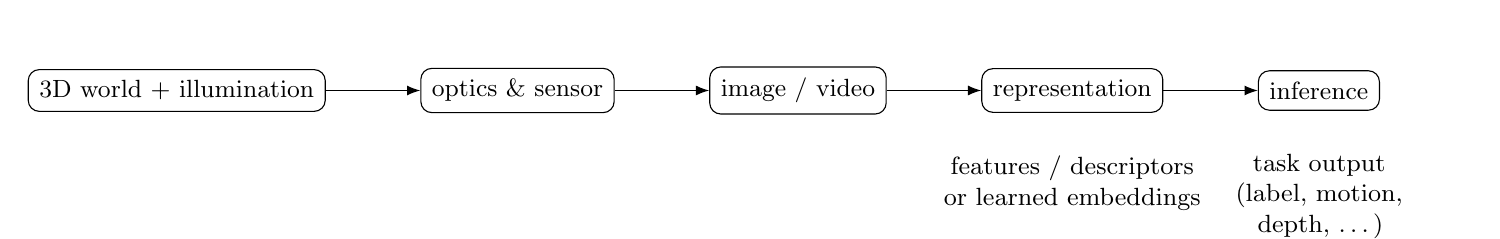
\begin{tikzpicture}[
  node distance=12mm,
  >=Latex,
  every node/.style={draw, rounded corners, inner sep=4pt, font=\small}
]
  \node (world) {3D world + illumination};
  \node[right=12mm of world] (sensor) {optics \& sensor};
  \node[right=12mm of sensor] (img) {image / video};
  \node[right=12mm of img] (repr) {representation};
  \node[right=12mm of repr] (inf) {inference};

  \draw[->] (world) -- (sensor);
  \draw[->] (sensor) -- (img);
  \draw[->] (img) -- (repr);
  \draw[->] (repr) -- (inf);

  \node[below=4mm of repr, draw=none, align=center, text width=40mm]
    {features / descriptors\\or learned embeddings};
  \node[below=4mm of inf, draw=none, align=center, text width=36mm]
    {task output\\(label, motion, depth, \dots)};
\end{tikzpicture}
\end{center}

\begin{intbox}
Vision is an \textbf{inverse problem}: many different 3D scenes can produce very similar (or identical) 2D images.
To do well, a system needs \textbf{assumptions} (priors) about the world.
\end{intbox}

\begin{itemize}
  \item \textbf{Information loss:} projection from 3D to 2D removes depth; occlusions hide parts of the scene.
  \item \textbf{Appearance variation:} illumination, viewpoint, shadows, specularities, and sensor noise change pixel values.
  \item \textbf{Local ambiguity:} textureless regions and repeated patterns make matching/motion ill-posed (aperture-style issues).
  \item \textbf{Scale and context:} what something \emph{is} may depend on global context rather than local pixels.
\end{itemize}

\subsection{Classical CV task landscape (big picture)}

The lecture highlights three core task families:
\begin{itemize}
  \item \textbf{Classification / recognition:} what is in the image? (object/category/scene labels).
  \item \textbf{Motion estimation and tracking:} how do pixels/objects move over time? (e.g., optical flow, tracking).
  \item \textbf{Scene reconstruction:} recover geometry (depth/3D structure) from one or multiple images.
\end{itemize}

\begin{notebox}
Many other tasks (segmentation, detection, pose estimation, SLAM) can be seen as combinations or refinements of the above
and will appear later in the course.
\end{notebox}

% ==========================================================
\section{Capturing Digital Images}

\subsection{Image formation models}

\subsubsection{Pinhole camera: perspective projection + trade-offs}

\begin{defbox}
A \textbf{pinhole camera} maps a 3D point $\vct{P}=(X,Y,Z)\T$ in camera coordinates to an image point
$\vct{p}=(x,y)\T$ by intersecting the ray from $\vct{P}$ through a single aperture (pinhole) with the image plane.
\end{defbox}

\begin{mathrule}
\textbf{Perspective projection (camera coordinates, image plane at distance $f$):}
\[
x = \frac{fX}{Z},\qquad y = \frac{fY}{Z}.
\]
\end{mathrule}

\begin{intbox}
\textbf{Trade-off (sharpness vs.\ brightness).}
A smaller pinhole yields a sharper image (less geometric blur) but lets in less light (darker image).
A larger pinhole is brighter but blurrier (rays from one scene point spread over an area).
\end{intbox}

\begin{notebox}
In practice we often use a \emph{virtual image plane in front of the pinhole} to avoid the ``flipped image'' mental picture;
the math stays the same.
\end{notebox}

\subsubsection{Projection models: perspective vs.\ orthographic/weak-perspective; vanishing points}

\begin{defbox}
\textbf{Perspective projection} scales by inverse depth $1/Z$ (farther objects appear smaller). \\
\textbf{Orthographic/Parallel projection} ignores depth scaling (reasonable if depth variation is small). \\
\textbf{Weak perspective (scaled orthographic)} approximates all depths in a region by a constant reference depth
$Z_0$ (e.g.\ the mean object depth), so perspective becomes a \emph{constant-scale} projection.
\end{defbox}

\begin{mathrule}
Let $(X,Y,Z)$ be camera coordinates and $(x,y)$ normalized image coordinates.

\begin{align*}
\textbf{Perspective:}\quad
& x = \frac{X}{Z}, \qquad y = \frac{Y}{Z}. \\[2pt]
\textbf{Weak perspective:}\quad
& \text{assume } Z = Z_0 + \Delta Z \text{ with } |\Delta Z|\ll Z_0 \\
& \Rightarrow\; x \approx \frac{X}{Z_0}, \qquad y \approx \frac{Y}{Z_0}
\quad \text{(constant scale within the region)} \\
\textbf{Orthographic/Parallel:}\quad
& x = X, \qquad y = Y
\quad \text{(optionally with a constant scale factor } s\text{).}
\end{align*}
\end{mathrule}

\begin{intbox}
\textbf{Vanishing points / horizon.}
In perspective projection, 3D parallel lines can meet at a \emph{vanishing point} in the image.
The \emph{horizon line} is the set of vanishing points for directions parallel to the ground plane.
In (weak) orthographic projection, parallel lines remain parallel (no vanishing points).
\end{intbox}

\begin{notebox}
\textbf{Orthographic/Parallel projection:} parallel 3D lines remain parallel in the image, so (in the ideal model) there are \textbf{no vanishing points}.
\end{notebox}

\begin{center}
  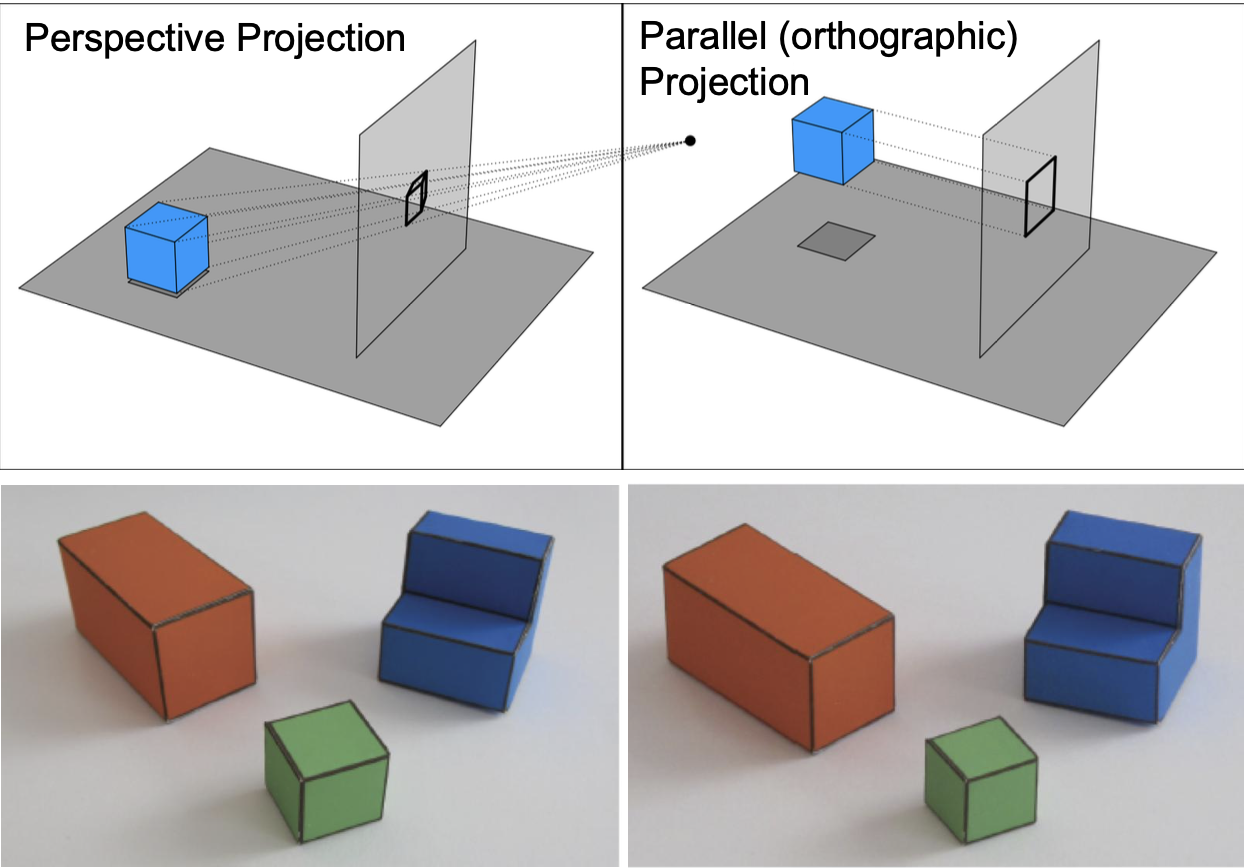
\includegraphics[width=0.7\linewidth]{projection.png}
\end{center}

\subsubsection{Thin lens model: focal length, focus, aperture}
\begin{notebox}
\textbf{Camera model note.} Despite using a thin lens for focusing/light collection, the mapping from 3D to 2D is still well-approximated by a \textbf{linear projective (pinhole) model}. More complex/thick lenses primarily require \textbf{non-linear distortion models} (calibration) in practice.
\end{notebox}

Real cameras use lenses to collect more light than a pinhole while keeping points approximately focused.

\begin{defbox}
\textbf{Focal length $f$:} distance from the (thin) lens center to the focal point where parallel incoming rays
(from infinity) converge.
\end{defbox}

\begin{intbox}
Although a lens is used for light collection and focusing, the \emph{geometric mapping} from 3D to 2D is still well
approximated by the same perspective projection equations as the pinhole model---the lens mainly improves brightness
by capturing rays from a finite solid angle.
\end{intbox}

\begin{defbox}
\textbf{Aperture:} an adjustable opening controlling the \emph{effective diameter} of the lens (how many rays are admitted).
\end{defbox}

\subsubsection{Depth of field and f-number (exposure vs.\ sharpness)}

\begin{defbox}
\textbf{Depth of field (DoF):} range of depths that appear acceptably sharp in the image.
\end{defbox}

\begin{mathrule}
\textbf{f-number / f-ratio (written as $f/N$):}\;
The \textbf{f-number} $N$ is a \emph{dimensionless} ratio
\[
N=\frac{f}{D}
\qquad\Longleftrightarrow\qquad
D=\frac{f}{N},
\]
where $f$ is the focal length and $D$ is the \emph{effective aperture diameter} (entrance pupil).
\end{mathrule}

\begin{itemize}
  \item \textbf{Larger $N$} (smaller aperture): \emph{less light} but \emph{larger DoF} (more of the scene appears sharp).
  \item \textbf{Smaller $N$} (larger aperture): \emph{more light} but \emph{smaller DoF} (stronger background blur).
\end{itemize}

\begin{exbox}
If $f=\SI{80}{mm}$ and $N=4$, then $D=f/N=\SI{20}{mm}$.
\end{exbox}

\begin{notebox}
Collected light is proportional to the \emph{aperture area}:
\[
\text{light} \propto D^2 \propto \frac{1}{N^2}.
\]
So changing the f-number by one full ``stop'' changes the light by roughly a factor of 2.
For two f-numbers $N_1,N_2$, the relative light is $\text{light}_1/\text{light}_2 \approx (N_2/N_1)^2$.
\end{notebox}

\begin{defbox}
\textbf{Geometric lens distortion} warps image geometry. Most important in CV: \textbf{radial distortion}
(barrel vs.\ pincushion), especially for wide FoV lenses. So most consumer cameras need calibration before being used in CV.
\end{defbox}

% ----------------------------------------------------------
\subsection{Digital sensors and the imaging pipeline}

\subsubsection{Sampling and quantization (resolution, aliasing, bit depth)}

\begin{defbox}
A digital image is a \textbf{discrete 2D function}:
\[
I:\{1,\dots,W\}\times\{1,\dots,H\}\to \{0,\dots,2^b-1\},
\]
where $b$ is the \textbf{bit depth} (e.g., $b=8$ for 256 intensity levels).
\end{defbox}

\begin{itemize}
  \item \textbf{Sampling} (finite pixel spacing) limits spatial resolution.
  \item \textbf{Aliasing} occurs when scene detail exceeds the sensor sampling rate (high frequencies fold into low ones).
  \item \textbf{Quantization} maps continuous irradiance to discrete intensity values; larger $b$ gives finer intensity steps.
\end{itemize}

\begin{notebox}
Anti-aliasing can be helped by optical blur (lens + sensor) or explicit low-pass filtering before downsampling.
\end{notebox}


\subsubsection{Noise sources and SNR intuition (shot/read noise; qualitative)}

\begin{defbox}
\textbf{Noise:} random variation in the measured pixel value under identical conditions.
In practice, \textbf{signal-to-noise ratio (SNR)} is often more informative than absolute noise.
\end{defbox}

\begin{itemize}
    \item \textbf{Shot noise:} photon counting statistics \textbf{(Poisson distributed)}. For large photon counts, Poisson is well-approximated by a Gaussian.
  \item \textbf{Read noise:} sensor/electronics noise (approximately signal-independent).
  \item \textbf{Exposure trade-off:} more exposure (time / aperture) increases signal and usually improves SNR, but may cause motion blur or saturation.
\end{itemize}

\begin{intbox}
Averaging multiple independent frames reduces noise variance (roughly $\propto 1/n$) and improves SNR.
\end{intbox}

\begin{notebox}
Many consumer cameras apply a \textbf{non-linear response} (gamma-like) to mimic human perception.
For CV, it is often beneficial to \textbf{linearize} intensities (invert the response) before photometric computations.
If you start from raw Bayer/CFA data, a common CV order is: \textbf{linearize raw CFA samples first, then demosaic} (so interpolation happens in a linear domain).
\end{notebox}


\subsubsection{Color filter arrays and demosaicing (Bayer pipeline overview)}

\begin{defbox}
Most sensors measure only \textbf{one} color per pixel using a \textbf{Color Filter Array (CFA)}.
The most common CFA is the \textbf{Bayer pattern} with twice as many green samples as red/blue. In a standard Bayer pattern: \textbf{50\% green, 25\% red, 25\% blue} (so the statement “50\% red…” is false).
\end{defbox}

\begin{itemize}
  \item Raw CFA data: each pixel has one channel (R/G/B).
  \item \textbf{Demosaicing} (debayering): interpolate missing channels from neighbors to obtain a full RGB image.
\end{itemize}

\begin{notebox}
More green samples reflect that perceived luminance is strongly influenced by green wavelengths; it also helps spatial detail.
\end{notebox}



\subsection{Color imaging}

\subsubsection{RGB vs.\ grayscale; white balance / color constancy (high-level)}

\begin{itemize}
  \item \textbf{Grayscale} is often sufficient for geometry/structure (edges, corners, motion) and can simplify modeling.
  \item \textbf{RGB} is useful when appearance cues matter (recognition, segmentation, materials).
\end{itemize}

\begin{defbox}
\textbf{White balance / color constancy (idea):}
compensate for the illuminant so that neutral objects appear neutral and colors are comparable across lighting conditions.
\end{defbox}

\subsection{Camera geometry and the camera matrix}

\subsubsection{Coordinate systems and homogeneous coordinates}

We distinguish:
\begin{itemize}
  \item \textbf{World coordinates} $\vct{P}_W=(X_W,Y_W,Z_W)\T$: fixed scene coordinate system.
  \item \textbf{Camera coordinates} $\vct{P}_C=(X_C,Y_C,Z_C)\T$: origin at the camera center, $Z_C$ points forward.
  \item \textbf{Image / pixel coordinates} $(u,v)$: discrete pixel grid on the sensor/image.
\end{itemize}

\begin{defbox}
\textbf{Homogeneous coordinates (idea):}
We often write points with an extra coordinate so that projections become linear.
\begin{itemize}
  \item 2D point $(x,y)$ becomes $\tilde{\vct{p}}=(x,y,1)\T$ (and also $(\lambda x,\lambda y,\lambda)\T$ is the same point for any $\lambda\neq 0$).
  \item 3D point $(X,Y,Z)$ becomes $\tilde{\vct{P}}=(X,Y,Z,1)\T$ (again defined only up to scale).
\end{itemize}
\end{defbox}

\subsubsection{Perspective projection + perspective division}

\begin{mathrule}
\textbf{Perspective division:}
If $\tilde{\vct{p}}=(x',y',w')\T$ is a homogeneous image point, then the Euclidean point is
\[
(x,y)=\left(\frac{x'}{w'},\frac{y'}{w'}\right).
\]
\end{mathrule}

\subsubsection{Extrinsics: pose as rotation and camera center}

\begin{defbox}
\textbf{Extrinsics (camera pose):}
They tell us \textbf{where the camera is} and \textbf{how it is oriented} relative to the world.
\begin{itemize}
  \item $\mat{R}$ is a \textbf{3D rotation matrix}. It rotates vectors without stretching or shearing.
        Concretely, $\mat{R}^\top \mat{R}=\mat{I}$ and $\det(\mat{R})=1$.
        (This set of valid 3D rotations is often called $SO(3)$.)
  \item $\vct{C}\in\R^3$ is the \textbf{camera center} in world coordinates (the camera position).
\end{itemize}
\end{defbox}

\begin{mathrule}
\textbf{World $\rightarrow$ camera:}
To express a world point in the camera coordinate system:
\begin{enumerate}
  \item shift the world point so the camera is at the origin: $\vct{P}_W - \vct{C}$
  \item rotate into the camera axes: multiply by $\mat{R}$
\end{enumerate}
\[
\vct{P}_C = \mat{R}\bigl(\vct{P}_W - \vct{C}\bigr).
\]
Often this is written as an affine form
\[
\vct{P}_C = \mat{R}\vct{P}_W + \vct{t},
\qquad
\vct{t} = -\mat{R}\vct{C}.
\]
\end{mathrule}

\subsubsection{Projection matrix (homogeneous form)}

\begin{mathrule}
\textbf{Pinhole camera model:}
\[
\tilde{\vct{p}} \sim \mat{P}\,\tilde{\vct{P}}_W,
\qquad
\mat{P} = \mat{K}\,[\mat{R}\mid \vct{t}].
\]
\end{mathrule}

\subsubsection{Intrinsics: $\mat{K}=(f_x,f_y,c_x,c_y,\text{skew})$}

\begin{defbox}
\textbf{Intrinsics} map from normalized camera coordinates to pixel coordinates, accounting for focal length in pixels
and sensor alignment.
\end{defbox}

\begin{mathrule}
A common intrinsic matrix form:
\[
\mat{K}=
\begin{pmatrix}
f_x & s   & c_x\\
0   & f_y & c_y\\
0   & 0   & 1
\end{pmatrix},
\]
where $(c_x,c_y)$ is the principal point, $s$ is skew (often $\approx 0$), and $f_x,f_y$ are focal lengths in pixel units.
\end{mathrule}

\begin{notebox}
In many calibration contexts, \textbf{intrinsics} are taken as $(\mat{K},\text{distortion coeffs})$, i.e., lens parameters (radial/tangential distortion) are grouped with intrinsics.
\end{notebox}

\subsection{Distortion and calibration}

\subsubsection{Learning-based calibration / rectification from ``in-the-wild'' images (idea)}
\begin{itemize}
  \item \textbf{Pixel-wise undistortion mapping:} learn a dense warp (e.g., U-Net predicts a per-pixel displacement / sampling grid).
  \item \textbf{Geometric cues:} infer intrinsics from vanishing points / horizon / line statistics (often combined with learning).
  \item \textbf{Direct regression:} CNN regresses intrinsics/extrinsics and/or distortion parameters from an image (often trained on synthetic distortions or pseudo-labels).
\end{itemize}

\subsubsection{Radial (and tangential) distortion models}

\begin{defbox}
\textbf{Geometric lens distortion:} The ideal pinhole model assumes rays travel perfectly straight. Real lenses bend light, often non-linearly near the edges, causing \textbf{radial distortion}.
\end{defbox}

\begin{mathrule}
\textbf{Radial distortion (``bulge'' around the center):}\;
Work in \textbf{normalized} image coordinates $(x,y)$ (i.e., after dividing by depth and removing $\mat{K}$).
Let $r^2 = x^2 + y^2$ be the squared distance from the image center.

Instead of a direct mapping, distortion scales the point's distance from the center using a polynomial:
\[
s(r)= 1 + k_1 r^2 + k_2 r^4 + k_3 r^6
\]
\begin{enumerate}
  \item Take the ideal, straight-ray coordinates: $(x, y)$
  \item Scale them by the distortion factor $s(r)$:
\end{enumerate}
\[
x_d = x\,s(r),\;\; y_d = y\,s(r).
\]
\end{mathrule}

\begin{itemize}
  \item \textbf{Barrel distortion ($k_1 < 0$):} Outer points are pulled \emph{inwards}. Straight lines bow outward like a barrel (typical for wide-angle/fisheye lenses).
  \item \textbf{Pincushion distortion ($k_1 > 0$):} Outer points are pushed \emph{outwards}. Straight lines bend inward like a pincushion (typical for telephoto lenses).
\end{itemize}

\subsubsection{Checkerboard calibration: reprojection error objective}

\begin{defbox}
\textbf{Camera calibration:} estimate intrinsics $\mat{K}$, distortion parameters, and (for each calibration image)
extrinsics $(\mat{R},\vct{t})$ by observing a known pattern (e.g., checkerboard).
\end{defbox}

\begin{mathrule}
\textbf{Reprojection error minimization:}
Instead of solving a direct equation, we guess the camera parameters and adjust them to minimize the error. For every known 3D corner on the checkerboard ($\vct{P}_i$):
\begin{enumerate}
 \item \textbf{Project:} Mathematically project the 3D point into the 2D image using our current guess for $\mat{K}$, distortion, $\mat{R}$, and $\vct{t}$. Let's call this computed pixel $\pi(\vct{P}_i)$.
 \item \textbf{Measure:} Find the actual pixel coordinates of that corner in the photograph ($\vct{p}_i$).
 \item \textbf{Compare:} Calculate the squared pixel distance between our guess and reality: $\norm{\vct{p}_i - \pi(\vct{P}_i)}^2$.
\end{enumerate}
We sum this error over all points $i$ and all calibration images $j$, and use an optimizer to find the parameters that minimize it:
\[
\min_{\mat{K},\,\text{dist},\,\{\mat{R}_j,\vct{t}_j\}}
\sum_{j}\sum_{i}\norm{\vct{p}_{i,j} - \pi(\mat{K},\text{dist},\mat{R}_j,\vct{t}_j;\vct{P}_i)}^2
\]
\end{mathrule}

\subsubsection{Interpreting calibration outputs (what parameters mean in practice)}

\begin{itemize}
  \item $\mat{K}$: focal lengths in pixels and principal point; sets the mapping between rays and pixel coordinates.
  \item Distortion coefficients: quantify how strongly pixels are warped away from the ideal pinhole model.
  \item Per-image $(\mat{R},\vct{t})$: pose of the calibration pattern relative to the camera.
\end{itemize}

\begin{notebox}
Calibration quality is often judged by the final RMS reprojection error (smaller is better),
but it must be interpreted together with image resolution and corner detection accuracy.
\end{notebox}


\subsubsection{Why calibration matters: enabling 3D reconstruction from multiple views}

\begin{intbox}
3D reconstruction from a single image is under-constrained.
With \textbf{multiple calibrated views}, geometry provides constraints that make depth estimation feasible
(epipolar geometry, stereo disparity, triangulation).
\end{intbox}

\begin{itemize}
  \item Accurate $\mat{K}$ and distortion correction are required for consistent multi-view geometry.
  \item Known relative poses $(\mat{R},\vct{t})$ allow mapping rays from different cameras into one common 3D frame.
\end{itemize}

\subsection{Active depth sensors and event cameras}

\subsubsection{Time-of-Flight (ToF) and LiDAR}
\begin{itemize}
  \item \textbf{ToF distance:} $d = \frac{c\,t}{2}$ (round-trip time $t$, speed of light $c$).
  \item \textbf{LiDAR:} ToF depth where a laser is emitted and the return time is measured (often with scanning).
\end{itemize}

\subsubsection{Event cameras (DVS)}
[Image comparing standard video frames vs event camera output]
\begin{itemize}
  \item \textbf{Standard cameras} capture full frames at a fixed rate (e.g., 30 FPS), recording redundant static background and suffering from motion blur on fast objects.
  \item \textbf{Event cameras (DVS)} work like the human optic nerve: each pixel operates independently and \emph{only fires an event when its brightness changes}.
  \item \textbf{Output:} An asynchronous stream of events $(x,y,t,\text{polarity})$.
  \item \textbf{Pros:} Microsecond temporal resolution, extremely low latency, no standard motion blur, and low bandwidth for static scenes.
\end{itemize}

% ==========================================================
\section{Digital Image Processing}

\subsection{Images as discrete signals}

\subsubsection{Neighborhoods, connectivity, boundary handling (padding/replication)}

\begin{defbox}
A grayscale image is a discrete 2D signal $I[n,m]$ on a pixel grid. Many operations use a local
\textbf{neighborhood} (e.g., $3\times 3$, $5\times 5$) around each pixel to compute an output.
\end{defbox}

Typical boundary handling when the neighborhood extends outside the image:
\begin{itemize}
  \item \textbf{Zero padding:} assume missing pixels are 0 (simple; can darken borders).
  \item \textbf{Replicate:} repeat boundary pixel values (often good for smoothing).
  \item \textbf{Reflect:} mirror the image at the boundary (often good for derivatives).
  \item \textbf{Circular / wrap:} treat image as periodic (matches FFT-based convolution).
\end{itemize}

\begin{notebox}
Border handling changes results near image edges. For FFT-based filtering you often pad the image
to avoid circular wrap-around artefacts.
\end{notebox}


\subsubsection{Correlation vs.\ convolution; shift-invariance and linearity}

\begin{defbox}
\textbf{Correlation} applies a kernel $h$ without flipping it:
\[
(y = x \star h)\quad\Rightarrow\quad
y[m,n] = \sum_{k,l} x[m+k,n+l]\;h[k,l].
\]
\textbf{Convolution} flips the kernel in both directions:
\[
(y = x * h)\quad\Rightarrow\quad
y[m,n] = \sum_{k,l} x[m+k,n+l]\;h[-k,-l].
\]
\end{defbox}

\begin{notebox}
Many CV libraries implement ``convolution'' routines that actually compute correlation
(because the kernel is learned/defined accordingly). Always check the convention.
\end{notebox}

\begin{intbox}
\textbf{Linear shift-invariant (LSI) viewpoint.}
Convolution is the prototypical LSI operation: linear combinations of inputs map to the same
linear combination of outputs, and shifting the input shifts the output.
\end{intbox}


\subsubsection{Convolution properties}
\begin{notebox}
Convolution is \textbf{linear}, \textbf{shift-invariant}, commutative, associative, and distributive.
\end{notebox}

\begin{exbox}
\textbf{Impulse response.} Convolving with an impulse kernel (1 at center, 0 elsewhere) leaves the image unchanged.
This is a useful sanity check for implementations.
\end{exbox}


% ----------------------------------------------------------
\subsection{Spatial filtering}

\subsubsection{Smoothing: box and Gaussian; separability and efficiency}

\begin{defbox}
A \textbf{low-pass filter} removes high-frequency components (fine details/noise), producing a smoother image.
\end{defbox}

\begin{defbox}
\textbf{Box filter:} Replaces each pixel by the average of its neighborhood.  \\
\textbf{Gaussian filter:} Weights central pixels higher, forming a bell curve.  \\
\textbf{Key facts:} Convolution of Gaussians is Gaussian; the Fourier transform of a Gaussian is Gaussian; and Gaussians are \textbf{separable}.
\end{defbox}

\subsubsection{Derivatives and edges: gradients \& Sobel}

\begin{mathrule}
\textbf{Finding Edges (Image Gradient):}
Edges are strong intensity changes. To find them, we compute the gradient vector for each pixel:
\begin{enumerate}
  \item \textbf{Horizontal change ($I_x$):} Convolve with a kernel like Sobel $K_x$ $\left(\begin{smallmatrix}-1&0&1\\-2&0&2\\-1&0&1\end{smallmatrix}\right)$. It literally subtracts the left neighbors from the right neighbors to find vertical edges.
  \item \textbf{Vertical change ($I_y$):} Convolve with $K_y=K_x^{\T}$ (subtracts top from bottom to find horizontal edges).
  \item \textbf{Edge Strength (Magnitude):} How stark is the contrast? $\norm{\nabla I} = \sqrt{I_x^2 + I_y^2}$
  \item \textbf{Edge Direction (Orientation):} Which way does the gradient point? $\theta = \operatorname{atan2}(I_y, I_x)$
\end{enumerate}
\end{mathrule}

\begin{notebox}
\textbf{Crucial:} Derivatives amplify noise. Always smooth the image first (e.g., with a Gaussian filter) before computing gradients!
\end{notebox}

\subsubsection{Second derivatives \& Unsharp Masking (Sharpening)}

\begin{defbox}
The \textbf{Laplacian} ($\Delta I = I_{xx} + I_{yy}$) measures how much a pixel differs from the average of its immediate neighbors. It highlights rapid changes and acts as a \textbf{high-pass filter}.
\end{defbox}

\begin{mathrule}
\textbf{Unsharp Masking (How to sharpen an image):}
\begin{enumerate}
  \item \textbf{Blur:} Smooth the original image to get $I_{\text{blur}}$ (removes fine details).
  \item \textbf{Extract Details:} Subtract the blur from the original to isolate the edges/high frequencies: $I_{\text{details}} = I - I_{\text{blur}}$.
  \item \textbf{Sharpen:} Add those details back to the original image, scaled by strength $\alpha$: $I_{\text{sharp}} = I + \alpha\,I_{\text{details}}$.
\end{enumerate}
\end{mathrule}

\begin{notebox}
\textbf{Exam pattern recognition:} 
1. Any kernel with a \textbf{large positive center} and \textbf{negative neighbors} (e.g., $\approx$ Impulse $-$ Gaussian) is a \textbf{sharpening filter}.
2. The discrete Laplacian kernel (e.g., center 4, neighbors -1) essentially performs this detail extraction in one step.
\end{notebox}

% ----------------------------------------------------------
\subsection{Frequency domain}
\subsubsection{Fourier transform intuition \& spectra}

\begin{defbox}
The Fourier transform decomposes an image into a sum of 2D sine/cosine waves. 
\begin{itemize}
  \item \textbf{Center (Low frequencies):} Smooth gradients, global illumination, basic shapes.
  \item \textbf{Edges (High frequencies):} Fine details, sharp edges, noise.
\end{itemize}
\end{defbox}

\begin{mathrule}
\textbf{Complex components of the spectrum:}
The transform produces complex numbers, yielding two meaningful parts:
\begin{enumerate}
  \item \textbf{Magnitude:} How \emph{strong} is a specific frequency? (Often visualized as the "spectrum" image).
  \item \textbf{Phase:} \emph{Where} are the structures located? Phase is far more important for preserving the spatial structure/intelligibility of an image than magnitude!
\end{enumerate}
\end{mathrule}

\begin{notebox}
\textbf{Exam heuristic:} An image with \textbf{more spatial detail/sharp edges} will have a spectrum with \textbf{energy spread further out from the center} (stronger high-frequency magnitude).
\end{notebox}

\subsubsection{Convolution theorem (filtering via multiplication in Fourier domain)}

\begin{mathrule}
\textbf{Convolution theorem:}\quad
\[
f = g*h\ \Longleftrightarrow\ F = G\cdot H,
\]
i.e., convolution in the spatial domain corresponds to multiplication in the Fourier domain
(and vice versa, products become convolutions).
\end{mathrule}

\begin{intbox}
For large kernels, FFT-based filtering can be faster:
pad image and kernel, take FFTs, multiply spectra, then inverse FFT.
\end{intbox}


\subsubsection{Sampling, aliasing, and Nyquist intuition}

\begin{defbox}
\textbf{Aliasing} occurs when sampling is too coarse: high frequencies ``fold'' into low frequencies.
To downsample safely, first low-pass filter (anti-alias filter), then subsample.
\end{defbox}


% ----------------------------------------------------------
\subsection{Multi-scale representations}
\subsubsection{Gaussian \& Laplacian Pyramids}

\begin{mathrule}
\textbf{Gaussian Pyramid (Progressive blurring):}
To build the next smaller level of the pyramid:
\begin{enumerate}
  \item \textbf{Smooth:} Apply a Gaussian filter to the current image (crucial to prevent aliasing!).
  \item \textbf{Downsample:} Throw away every second row and column.
\end{enumerate}
Result: A set of increasingly small, blurred images (low-pass).
\end{mathrule}

\begin{mathrule}
\textbf{Laplacian Pyramid (Storing the lost details):}
To capture exactly what details were lost when moving to a smaller Gaussian level:
\begin{enumerate}
  \item \textbf{Upsample:} Take the smaller, blurry Gaussian level and double its size (interpolate).
  \item \textbf{Subtract:} Subtract this upsampled blurry image from the original, higher-resolution Gaussian level.
\end{enumerate}
Result: A set of "detail images" (band-pass). You can perfectly reconstruct the original image by adding the details back layer by layer.
\end{mathrule}

\begin{notebox}
\textbf{Difference of Gaussians (DoG):} If you subtract two differently blurred images of the \emph{same size}, you approximate the Laplacian-of-Gaussian (LoG). This is the foundation of SIFT feature detection!
\end{notebox}

\begin{center}
  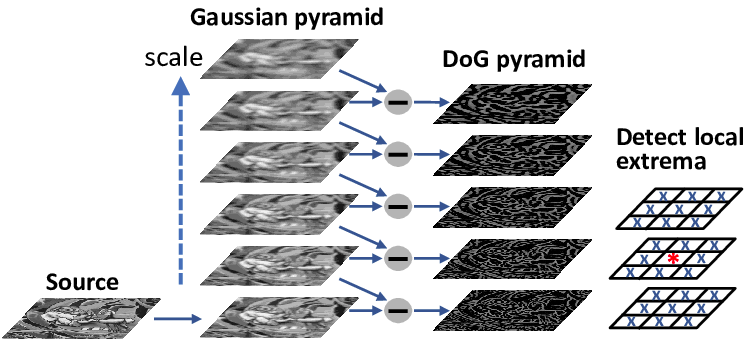
\includegraphics[width=0.8\linewidth]{DoG.png}
\end{center}
% ----------------------------------------------------------
\subsection{Inverse problems}
\subsubsection{Blur models and the failure of naive inverse filtering}

\begin{defbox}
\textbf{The problem:} We observe a blurry, noisy image $y$. We want to recover the sharp original $x$.
Model: \quad $y = x*h + \text{noise}$ \quad (where $h$ is the Point Spread Function / blur kernel).
\end{defbox}

\begin{mathrule}
\textbf{Naive inverse filtering:}
Since spatial convolution is Fourier multiplication ($Y = X \cdot H + N$), the naive approach is to just divide in the frequency domain:
\[
\text{Guess: } \hat{X} = \frac{Y}{H} = X + \frac{N}{H}
\]
\textbf{Why this fails:} Blur kernels $H$ typically destroy high frequencies, meaning $H \approx 0$ for high frequencies. Dividing the noise $N$ by a number close to zero causes the term $\frac{N}{H}$ to \textbf{explode}, completely burying the image in amplified noise.
\end{mathrule}


\subsubsection{Regularization intuition (Wiener / Lucy--Richardson / blind deconvolution overview)}

\begin{intbox}
\textbf{Regularization} stabilizes inversion by trading off data fidelity and smoothness/prior assumptions.
Instead of dividing by tiny $H$, we damp problematic frequencies.
\end{intbox}

Mentioned classical options (know the idea and when they are used):
\begin{itemize}
  \item \textbf{Wiener filter:} frequency-dependent trade-off using noise/signal statistics (conceptual).
  \item \textbf{Regularized filters:} add penalties (e.g., Tikhonov) to avoid unstable solutions.
  \item \textbf{Lucy--Richardson:} iterative deconvolution (often for Poisson noise; concept).
  \item \textbf{Blind deconvolution:} estimate both $x$ and $h$ (harder; needs priors/constraints).
\end{itemize}


% ----------------------------------------------------------
\subsection{Gradient-domain processing}

\subsubsection{Gradients as a vector field; integrability and curl intuition}

\begin{defbox}
The image gradient field
\[
\vct{v} = (I_x, I_y)
\]
can be seen as a \textbf{vector field} over pixels.
If $\vct{v}$ is exactly a gradient of some image, it is \textbf{integrable} (conservative) and has (discrete) curl $\approx 0$.
\end{defbox}

\begin{notebox}
After editing a gradient field (e.g., mixing gradients from different images), it typically becomes non-conservative
(non-zero curl), so direct integration fails.
\end{notebox}


\subsubsection{Poisson reconstruction (why it appears, when it works)}

\begin{mathrule}
\textbf{Poisson reconstruction (core idea):}\;
Given a desired vector field $\vct{v}=(v_x,v_y)$, recover an image $I$ whose gradients match $\vct{v}$
in least-squares sense:
\[
\min_I \sum_{m,n} \|\nabla I[m,n] - \vct{v}[m,n]\|^2
\quad\Longrightarrow\quad
\Delta I = \nabla\cdot \vct{v},
\]
a 2D Poisson equation with boundary conditions.
\end{mathrule}

\begin{intbox}
Think of this as: \emph{choose the image whose gradients are as close as possible to what we want.}
The Laplacian $\Delta I$ is the divergence of the gradient, so it naturally appears in the normal equations.
\end{intbox}


\subsubsection{Applications: blending, reflection removal, stitching/editing, tone/HDR compression}

Common gradient-domain applications (as motivated in the lecture):
\begin{itemize}
  \item \textbf{Seamless blending (Poisson blending):} paste an object while matching surrounding gradients.
  \item \textbf{Image fusion / reflection removal:} keep strong gradients from the desired layer, suppress others.
  \item \textbf{Stitching/editing:} reduce seams by enforcing consistent gradients across overlaps.
  \item \textbf{HDR/tone manipulation:} modify gradient magnitudes to compress dynamic range while preserving structure.
\end{itemize}


% ----------------------------------------------------------
\subsection{CNN note connecting DIP to learning}
\subsubsection{Transposed convolution as upsampling}

\begin{mathrule}
\textbf{Transposed Convolution ("Learned Upsampling"):}
Often confusingly called "deconvolution", it is \emph{not} the inverse of a convolution, but a convolution applied to an artificially inflated input.
\textbf{How it works (Mental Model):}
\begin{enumerate}
  \item \textbf{Stretch:} Take the input grid and insert $s-1$ zeros between every pixel (where $s$ is the stride).
  \item \textbf{Pad:} Adjust the edges by subtracting padding $2p$.
  \item \textbf{Convolve:} Slide a standard kernel of size $k$ over this new, sparse grid.
\end{enumerate}
\textbf{Output size formula:}
\[
\text{out} = (\text{in}-1)\cdot s - 2p + k
\]
\end{mathrule}

% ==========================================================
\section{Machine Learning}

\begin{notebox}
\textbf{ML as design choices.}
Training a model means choosing (i) hypothesis space/model class, (ii) objective/loss,
and (iii) an optimizer. Deep learning shifts much of the feature-design burden into learning,
but the choices still matter in practice.
\end{notebox}

\subsection{Dimensionality reduction}
\subsubsection{Motivation: compress $d$-dimensional data to $k<d$ with minimal information loss}
High-dimensional image/feature vectors often lie near a lower-dimensional manifold/subspace.
Reducing dimensionality can:
(i) denoise, (ii) compress, (iii) make learning easier (less overfitting), (iv) enable visualization.

\begin{intbox}
\textbf{Geometric picture:} find a low-dimensional subspace such that when you project the data onto it,
the projected points are still ``spread out'' as much as possible.
\end{intbox}

\subsubsection{PCA: Principal Component Analysis}


\begin{mathrule}
\textbf{How to compute PCA (The Recipe):}
Goal: Find a new set of axes (directions) that maximize the variance/spread of the data.
\begin{enumerate}
  \item \textbf{Center the data:} Subtract the mean $\bar{\vct{x}}$ from all data points.
  \item \textbf{Covariance:} Compute the covariance matrix $\mat{C} = \frac{1}{n}\mat{X}^\top\mat{X}$.
  \item \textbf{Eigen-decomposition:} Find the eigenvectors and eigenvalues of $\mat{C}$.
\end{enumerate}
\textbf{Interpretation:}
\begin{itemize}
  \item \textbf{Eigenvectors:} The new axes (Principal Directions).
  \item \textbf{Eigenvalues:} The amount of variance captured along that axis.
\end{itemize}
\textbf{Dimensionality reduction:} Sort eigenvectors by highest eigenvalue and keep only the top-$k$ vectors. Throw away small eigenvalues (often just noise).
\end{mathrule}

\subsubsection{Example: Eigenfaces (images as points in \texorpdfstring{$\mathbb{R}^{NM}$}{R^{NM}})}
Flatten an $N\times M$ image into a vector in $\R^{NM}$. PCA on a set of face images yields:
\begin{itemize}
  \item \textbf{Mean face} $\bar{\vct{x}}$.
  \item \textbf{Eigenfaces} $\{\vct{v}_1,\dots,\vct{v}_k\}$ (principal directions).
\end{itemize}

\begin{mathrule}
\textbf{Projection / reconstruction:}
\[
\vct{a} = \mat{V}_k^\top (\vct{x}-\bar{\vct{x}}),
\qquad
\hat{\vct{x}} = \bar{\vct{x}} + \mat{V}_k \vct{a},
\]
where $\mat{V}_k=[\vct{v}_1,\dots,\vct{v}_k]$.
\end{mathrule}

\begin{exbox}
\textbf{Recognition idea (classic):} project a test face to PCA coefficients $\vct{a}$ and do nearest-neighbor
matching in coefficient space. Works if training variation matches test variation; fails under large changes
(illumination/pose/expression) unless handled explicitly.
\end{exbox}

\begin{notebox}
\textbf{Exam implication.} Therefore the claim “Eigenface-based recognition is highly robust to extreme lighting/pose/expression changes” is \textbf{incorrect}.
\end{notebox}

\subsection{Deep learning for images: CNN essentials}
\subsubsection{Convolution layer computation}

A convolution layer applies $K$ learned filters to an input tensor $\mat{X}\in\R^{H\times W\times C}$.
\begin{mathrule}
\textbf{How a Filter works (3D Sliding Dot Product):}
For each position in the image:
\begin{enumerate}
  \item \textbf{Extract a 3D patch:} Take a chunk of the image that matches the filter's spatial size ($k \times k$) across \emph{all} input channels $C$.
  \item \textbf{Dot Product:} Multiply every pixel value in the patch with the corresponding filter weight, and sum it all up into a \emph{single number}.
  \item \textbf{Add Bias:} Add a learned scalar bias $b$.
\end{enumerate}
This resulting single number becomes one pixel in the output feature map. Since we slide the \emph{exact same filter} over the whole image, we get \textbf{translation equivariance} (shifting the input shifts the output).
\end{mathrule}

\begin{center}
  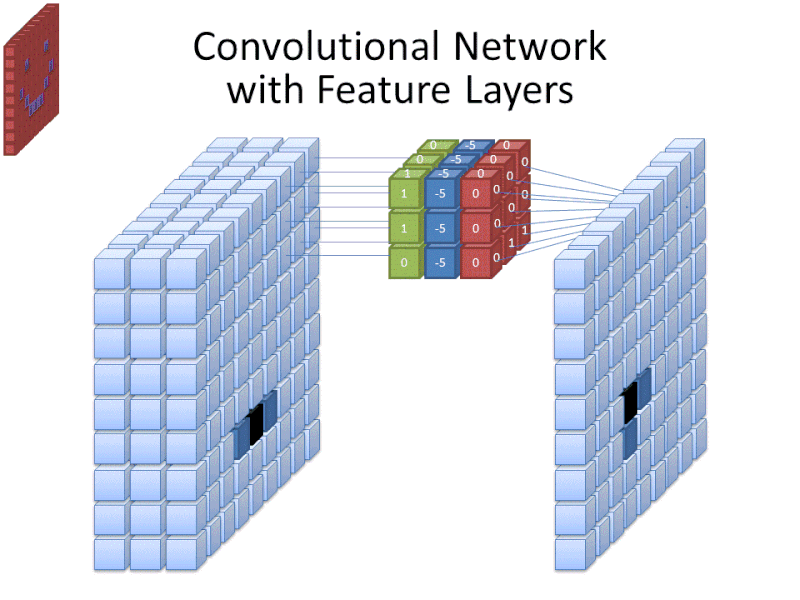
\includegraphics[width=0.5\linewidth]{3d_conv.png}
\end{center}

\begin{mathrule}
\textbf{Exam Math: CNN Dimensions \& Parameters}

\textbf{1. Output Spatial Size:}
\[
\text{Size}_{\text{out}} = \Big\lfloor\frac{\text{Size}_{\text{in}} + 2 \times \text{padding} - \text{kernel\_size}}{\text{stride}}\Big\rfloor + 1
\]

\textbf{2. Number of Parameters (Weights):}
\[
\text{Params} = (\text{kernel\_width} \times \text{kernel\_height} \times \text{Channels}_{\text{in}} + \text{bias}) \times \text{Filters}_{\text{out}}
\]
\textit{(Note: bias is usually $1$ per filter, so add $+1$ inside the parenthesis if bias is used).}
\end{mathrule}

\begin{exbox}
\textbf{Exam Examples:}\\
\textbf{Size:} Input $32\times 32$, $7\times 7$ conv, $s=1, p=0 \Rightarrow 26\times 26$. Three such layers in a row: $32 \to 26 \to 20 \to 14$.\\
\textbf{Params:} Input has 3 channels. We use 16 filters of size $3\times 3$ (no bias). Each filter has $3 \times 3 \times 3 = 27$ weights. Total parameters: $16 \times 27 = 432$.
\end{exbox}

\begin{intbox}
\textbf{Template matching view:} a filter responds strongly where local image content matches the learned kernel.
\end{intbox}

\subsubsection{Nonlinearities (e.g., ReLU) and pooling/downsampling}
\begin{defbox}
\begin{itemize}
  \item \textbf{ReLU:} $f(x)=\max(0,x)$ introduces non-linearity and sparsity.
  \item \textbf{Pooling (e.g., max-pool):} downsample feature maps; more robustness to small translations,
  reduces computation, increases receptive field.
\end{itemize}
\end{defbox}

\subsubsection{Stride/padding and the notion of receptive field}
\begin{itemize}
  \item \textbf{Stride:} step size of the kernel; larger stride $\Rightarrow$ downsampling.
  \item \textbf{Padding:} how boundaries are handled; ``same'' padding keeps spatial resolution.
  \item \textbf{Receptive field:} region of input that influences one output activation; grows with depth and pooling.
\end{itemize}

\begin{qbox}
\textbf{Common exam pitfall:} convolution gives \emph{translation equivariance}, not full translation invariance.
Pooling/aggregation is what increases invariance to small shifts.
\end{qbox}

\subsubsection{From features to class scores: (simple) classifier head intuition}
A typical classifier CNN ends with:
\begin{itemize}
  \item spatial aggregation (flatten / global average pooling),
  \item fully connected layer(s),
  \item class scores (logits) $\rightarrow$ softmax probabilities.
\end{itemize}

\subsubsection{Classification with convolution (bridge to dense prediction)}

\begin{intbox}
A convolution kernel computes a weighted sum over a local patch and produces a strong response
where the patch matches the kernel.
This can be used not only for whole-image classification but also for \emph{dense} prediction:
e.g.\ predicting the class of the \emph{center pixel} from its neighborhood.
This viewpoint connects CNNs naturally to semantic segmentation (later lecture).
\end{intbox}

% ==========================================================
\section{Feature Extraction}

\subsection{Why features? Robustness and invariances}

\begin{notebox}
\textbf{Lecture intuition:}
early visual processing decomposes the input into features (color differences, local edges/textures, motion).
Higher-level pattern perception groups them into contours/regions.
Attention and working memory strongly limit what is processed deeply.
\end{notebox}

\subsubsection{What makes a ``good'' feature: repeatability, distinctiveness, robustness}
\begin{defbox}
A good local feature is:
\begin{itemize}
  \item \textbf{Repeatable:} detected at the same physical scene point across views/conditions.
  \item \textbf{Distinctive:} descriptor discriminates it from others (few false matches).
  \item \textbf{Robust:} stable under noise, blur, illumination changes, modest viewpoint changes.
  \item \textbf{Efficient:} computable and matchable at scale.
\end{itemize}
\end{defbox}

\subsection{Model-based vs.\ learning-based feature extraction (framing)}
\subsubsection{Model-based pipeline: detect $\rightarrow$ describe $\rightarrow$ match}
\begin{intbox}
\textbf{Classic local-feature pipeline:}
\[
\text{detect keypoints} \ \rightarrow\ \text{compute descriptor}\ \rightarrow\ \text{match descriptors}.
\]
Used in registration, panorama stitching, SfM, retrieval.
\end{intbox}

\subsubsection{Model-based image classification with local features (BoVW + pooling)}

\begin{mathrule}
\textbf{BoVW Pipeline (The Recipe):}
Instead of matching individual features, we represent the whole image as a frequency histogram of "visual words".
\begin{enumerate}
  \item \textbf{Extract:} Find keypoints and compute local descriptors (e.g., SIFT) across all training images.
  \item \textbf{Build Vocabulary:} Group all these descriptors into $K$ clusters using $k$-means. The cluster centers are your "visual words".
  \item \textbf{Encode Image:} For a new image, extract its descriptors and assign each one to the nearest visual word (hard assignment).
  \item \textbf{Pool:} Count the frequencies of each word to form a single $K$-dimensional histogram for the entire image.
  \item \textbf{Classify:} Feed this single histogram vector into a standard classifier (e.g., SVM).
\end{enumerate}
\end{mathrule}

\begin{intbox}
This is a useful conceptual bridge to CNNs:
CNNs \emph{learn} filters end-to-end, and pooling appears there as well to gain robustness.
\end{intbox}

\subsubsection{Learning-based idea: features learned to minimize task loss}
Instead of manually designing kernels/descriptors, CNNs learn filter banks from data via backprop:
features become task-adapted (classification/detection/segmentation).

\subsection{Invariances emphasized in the lecture}
\subsubsection{Shift-invariance: convolution with useful kernels}
\begin{itemize}
  \item Many hand-crafted filters are translation-equivariant detectors (Gaussian smoothing, derivatives, Laplacian).
  \item In CNNs, learned convolution kernels provide translation-equivariant feature extraction.
\end{itemize}

\subsubsection{Scale-invariance: image pyramids / scale space}
Scale changes are ubiquitous in images (objects at different distances).
Classic solution: \textbf{explicit multi-scale} processing (pyramids / scale space).

\subsection{SIFT (Scale-Invariant Feature Transform)}
\subsubsection{The SIFT Pipeline}
\begin{enumerate}
  \item \textbf{Scale space (DoG):} Build Gaussian pyramid and compute Difference-of-Gaussians ($D(\vct{x},\sigma)=G(k\sigma)-G(\sigma)$) to approximate LoG.
  \item \textbf{Keypoint detection:} Find local extrema of DoG in 3D neighborhood (space + scale).
  \item \textbf{Filtering:} Reject low-contrast (noise) and unstable (edge) points.
  \item \textbf{Orientation assignment:} Find dominant gradient orientation peak to normalize rotation.
  \item \textbf{Descriptor construction:} Take patch aligned to orientation, split into $4\times4$ tiles. Build 8-bin gradient histogram per tile $\Rightarrow \mathbf{128\text{-D}}$ descriptor. Normalize for illumination.
  
\end{enumerate}
\begin{qbox}
SIFT is designed to be robust to \textbf{(i)} translation (locality), \textbf{(ii)} scale (scale space),
\textbf{(iii)} rotation (orientation assignment), and moderately to illumination (normalization).
It is \emph{not} fully invariant to large viewpoint changes or heavy blur/occlusion.
\end{qbox}

\subsubsection{Matching intuition (nearest neighbor in descriptor space; typical failure modes)}
Match by nearest neighbor (e.g., Euclidean distance).
Common heuristic: ratio test (best vs.\ second-best distance) to reject ambiguous matches.
Failure modes: repetitive textures, large viewpoint changes, significant appearance changes.

\subsection{CNN features as descriptors (as shown)}
\subsubsection{Using intermediate activations as mid-/high-level features}
\begin{itemize}
  \item Early layers: edges/textures (low-level). \textbf{Exam fact:} Here you expect to find learned filter kernels that approximate Gaussians.
  \item Middle layers: parts/patterns (mid-level).
  \item Deep layers: semantic concepts (high-level).
\end{itemize}
Intermediate feature maps can serve as descriptors for tasks beyond classification (e.g., transfer learning, retrieval, style).

\subsubsection{Architecture milestones (AlexNet $\rightarrow$ VGG $\rightarrow$ ResNet / GoogLeNet overview)}
\begin{itemize}
  \item \textbf{AlexNet (2012):} established modern deep CNNs for large-scale classification.
  \item \textbf{VGG (2014):} deeper stacks of small ($3\times3$) convolutions.
  \item \textbf{GoogLeNet/Inception (2015):} multi-branch modules for efficiency.
  \item \textbf{ResNet (2016):} residual connections enable very deep networks.
\end{itemize}

\begin{notebox}
\textbf{Top-5 error rate (ImageNet-style).}
A prediction is counted as correct if the true label is among the top-5 predicted classes
(so \emph{error} means it is not in the top 5). \\
\textbf{Exam fact:} ResNet can achieve a better top-5-error rate than humans.
\end{notebox}

% ==========================================================
\section{Segmentation}

\subsection{What is segmentation? Types and applications}

\subsubsection{Semantic vs.\ instance vs.\ panoptic segmentation}

\begin{defbox}
\textbf{Segmentation} = partition an image into \textbf{groups of pixels that belong together}.
The output is a label per pixel (a mask), not just a single label for the whole image.
\end{defbox}

\begin{itemize}
  \item \textbf{Semantic segmentation:} assigns a \emph{class label} to every pixel (all ``car'' pixels share the same label).
  \item \textbf{Instance segmentation:} separates \emph{individual object instances} (car \#1 vs.\ car \#2).
  \item \textbf{Panoptic segmentation:} combines both: semantic classes \emph{and} instance IDs where applicable.
\end{itemize}

\begin{notebox}
Relationship to other tasks (big picture): classification has \emph{no spatial extent}; detection outputs boxes; segmentation outputs \emph{pixel masks}.
\end{notebox}

\subsubsection{Examples (editing, autonomous driving, medical imaging)}
\begin{itemize}
  \item \textbf{Image editing:} select foreground/background, object cutout, content-aware manipulation.
  \item \textbf{Autonomous driving:} road, lane, sidewalk, cars, pedestrians (scene understanding).
  \item \textbf{Medical imaging:} organs/tumors/lesions for measurement and diagnosis support.
\end{itemize}

\subsubsection{Why segmentation is hard (ambiguity, boundaries, annotation cost)}
\begin{intbox}
Segmentation is hard because \textbf{pixels are ambiguous}: boundaries may be weak/blurred, objects can have similar color/texture,
and occlusions hide parts. For learning, dense pixel labels are \textbf{expensive} to annotate.
\end{intbox}

\begin{itemize}
  \item \textbf{Boundary ambiguity:} smooth transitions, motion blur, low contrast edges.
  \item \textbf{Appearance ambiguity:} same object can look different under illumination; different objects can look similar.
  \item \textbf{Scale/context:} class decisions may require global context (e.g., ``road'' vs.\ ``wall'' texture locally).
\end{itemize}

\begin{qbox}
\textbf{Exam pitfall:} do not confuse \emph{semantic segmentation} (pixel-wise class labels) with \emph{instance segmentation} (separate object IDs).
\end{qbox}


\subsection{Segmentation by clustering}

\subsubsection{Pixels as points in feature space (color, color+location)}
\begin{defbox}
Model-based idea: represent each pixel $i$ as a feature vector $\vct{x}_i$ and cluster pixels in feature space.
\end{defbox}

Typical choices:
\begin{itemize}
  \item Color only: $\vct{x}_i = (R_i,G_i,B_i)\in\R^3$.
  \item Color + location (encourages spatial coherence): $\vct{x}_i = (R_i,G_i,B_i,u_i,v_i)\in\R^5$.
\end{itemize}

\begin{notebox}
Adding $(u,v)$ helps avoid grouping distant pixels that merely share color.
Often you need to \textbf{scale/normalize} color vs.\ position so neither dominates distances.
\end{notebox}

\subsubsection{K-means clustering (algorithm + typical failure modes)}
\begin{defbox}
\textbf{$k$-means} partitions $\{\vct{x}_i\}_{i=1}^N$ into $k$ clusters by minimizing within-cluster squared distances.
\end{defbox}

\begin{mathrule}
\textbf{$k$-means objective:}\quad
\[
\min_{\{\mathcal{C}_1,\dots,\mathcal{C}_k\}} \ \sum_{c=1}^k \sum_{i\in\mathcal{C}_c} \|\vct{x}_i - \vct{\mu}_c\|^2,
\qquad
\vct{\mu}_c = \frac{1}{|\mathcal{C}_c|}\sum_{i\in\mathcal{C}_c}\vct{x}_i.
\]
\end{mathrule}

Algorithm (as used in the lecture):
\begin{enumerate}
  \item Initialize $k$ cluster centers (often random).
  \item Assign each point to the nearest center.
  \item Recompute each center as the mean of its assigned points.
  \item Repeat until centers stop changing.
\end{enumerate}

Typical failure modes:
\begin{itemize}
  \item \textbf{Needs $k$:} must choose number of segments.
  \item \textbf{Initialization sensitivity:} different starts $\Rightarrow$ different results (local minima).
  \item \textbf{Not boundary-aware:} clusters by feature similarity, not by edges; can ``bleed'' across boundaries.
\end{itemize}


\subsection{Segmentation with graphs}

\subsubsection{Pixels as nodes; affinity weights and neighborhoods}
\begin{defbox}
Graph-based idea: build a graph $G=(V,E)$ where nodes are pixels (or superpixels).
Edges connect neighbors; weights encode similarity.
\end{defbox}

\begin{itemize}
  \item Node set: $V=\{1,\dots,N\}$.
  \item Neighborhood edges: $(i,j)\in E$ typically for 4- or 8-neighborhood (or within a radius).
  \item Affinity weight $a_{ij}$ is large if pixels are similar (e.g., similar color and close in space).
\end{itemize}

\begin{notebox}
The affinities can be stored in an \textbf{affinity matrix} $\mat{A}\in\R^{N\times N}$ (often sparse),
with $\mat{A}_{ij}=a_{ij}$ and typically $\mat{A}$ symmetric.
\end{notebox}

\subsubsection{Spectral/eigenvector-based clustering}

\begin{mathrule}
\textbf{Spectral Clustering (Intuition \& Math):}
Instead of clustering pixels in coordinate space, we cluster them based on how they are connected in a graph.
\begin{enumerate}
  \item \textbf{Affinity Matrix ($\mat{A}$):} Build a matrix where $A_{ij}$ is high if pixel $i$ and $j$ are similar (e.g., in color and distance).
  \item \textbf{The Goal:} Find a group assignment vector $\vct{w}$ that maximizes the connections \emph{within} the group: $\max (\vct{w}\T \mat{A}\vct{w})$.
  \item \textbf{The Solution:} Mathematically, maximizing this quadratic form (with a normalized $\vct{w}$) is exactly solved by finding the \textbf{eigenvectors} corresponding to the largest eigenvalues of $\mat{A}$ (or the Graph Laplacian).
\end{enumerate}
\end{mathrule}

Algorithm sketch from the slides:
\begin{enumerate}
  \item Construct affinity matrix $\mat{A}$.
  \item Compute eigenvalues/eigenvectors.
  \item Use eigenvectors to form memberships (e.g., thresholding on an eigenvector or a derived score).
  \item Remove clustered elements (zero out corresponding rows/cols in $\mat{A}$); repeat.
\end{enumerate}

\begin{notebox}
\textbf{Exam stopping rule.} If you iteratively extract one cluster per round and stop when the \emph{largest} eigenvalue drops below a threshold, then
\[
\#\text{clusters} = \#\{\text{rounds with } \lambda_{\max} \ge \text{threshold}\}.
\]
\end{notebox}

\subsubsection{Graph Cut \& GrabCut}

\begin{mathrule}
\textbf{Graph Cut (Energy Minimization):}
Segmentation is framed as assigning a label $y_i$ (e.g., foreground or background) to each pixel to minimize an overall "energy" cost:
\[
E(\vct{y}) = \underbrace{\sum_i D_i(y_i)}_{\text{Data term}} \;+\; \lambda \underbrace{\sum_{(i,j)\in E} V_{ij}(y_i,y_j)}_{\text{Smoothness term}}
\]
\begin{itemize}
  \item \textbf{Data term (Likelihood):} Cost of assigning a pixel to a label. (Does this pixel look more like the background or foreground color model?)
  \item \textbf{Smoothness term (Boundary):} Penalizes assigning different labels to neighboring pixels, \emph{unless} there is a strong, natural image edge between them.
\end{itemize}
This global optimum is efficiently found using \textbf{min-cut/max-flow} algorithms.
\end{mathrule}

\begin{notebox}
\textbf{GrabCut (The application):} An interactive tool using Graph Cuts. The user draws a rough bounding box. The algorithm builds Gaussian Mixture Models (GMMs) for foreground/background, runs min-cut, updates the GMMs based on the new mask, and repeats iteratively.
\end{notebox}


\subsection{Segmentation by fitting}
\subsubsection{Parametric shapes and voting}
\begin{defbox}
If segments correspond to known \textbf{parametric shapes} (lines, circles, etc.),
we can detect them by searching in the \textbf{parameter space} of that shape family.
\end{defbox}

\subsubsection{Hough transform (lines/circles as main example)}
\begin{defbox}
\textbf{Hough transform} = voting scheme: edge pixels vote for shape parameters; peaks in an accumulator indicate shapes.
\end{defbox}

Line example (robust to vertical lines):
\begin{mathrule}
\textbf{Line parameterization:}\quad
\[
\rho = x\cos\theta + y\sin\theta.
\]
Each edge pixel $(x,y)$ votes for all $(\rho,\theta)$ pairs consistent with it.
\end{mathrule}

Procedure:
\begin{enumerate}
  \item Run an \textbf{edge detector} (to reduce points).
  \item For each edge pixel, vote in an accumulator $H(\rho,\theta)$.
  \item Find \textbf{peaks} $H(\rho,\theta) > T$ (threshold / peak finding).
  \item Convert peak parameters back to lines in the image.
\end{enumerate}

\begin{notebox}
Dimensionality: the Hough space dimension equals the number of free parameters of the shape.
Typical cases:
\begin{itemize}
  \item \textbf{2D line:} 2 parameters $(\rho,\theta)$.
  \item \textbf{2D circle:} 3 parameters $(x_0,y_0,r)$ (only 2D if $r$ is fixed/known).
  \item \textbf{2D ellipse:} \textbf{5 parameters} $(x_0,y_0,a,b,\theta)$ \textbf{(so 5D Hough space)}.
  \item \textbf{3D plane:} 3 parameters (e.g.\ unit normal + distance).
  \item \textbf{3D ellipsoid:} typically \textbf{9 parameters} (center 3 + axes 3 + orientation 3), not 5 unless heavily constrained.
\end{itemize}
More parameters $\Rightarrow$ larger accumulator and higher cost.
\end{notebox}


\subsection{Segmentation by learning}

\subsubsection{Pixelwise classification with paired training data}
\begin{defbox}
Learning-based semantic segmentation uses \textbf{paired training data}:
for each training image, \textbf{each pixel has a class label}. At test time, the model predicts a label for every pixel.
\end{defbox}

\subsubsection{CNN/FCN idea: per-pixel scores and argmax predictions}
\begin{intbox}
Core idea (from the slides): encode the whole image with a CNN and produce \textbf{per-pixel class scores}
(\emph{fully convolutional} / FCN-style). Then pick the best class by $\argmax$ at each pixel.
\end{intbox}

\begin{mathrule}
\textbf{Score-tensor view (two variants):}\quad
\[
\underbrace{3\times H\times W}_{\text{input}}
\ \xrightarrow{\text{only convs (no downsampling)}}\
\underbrace{C\times H\times W}_{\text{scores}}
\ \xrightarrow{\argmax}\
\underbrace{H\times W}_{\text{labels}}.
\]
\[
\underbrace{3\times H\times W}_{\text{input}}
\ \xrightarrow{\text{encoder (down)}}\
\underbrace{C\times H'\times W'}_{\text{scores}}
\ \xrightarrow{\text{decoder (up)}}\
\underbrace{C\times H\times W}_{\text{scores}}
\ \xrightarrow{\argmax}\
\underbrace{H\times W}_{\text{labels}}.
\]
\end{mathrule}

\subsubsection{Resolution mismatch problem (downsampling vs.\ dense output)}
\begin{defbox}
Classification CNNs often downsample aggressively (pooling/stride) to gain receptive field and efficiency,
but segmentation needs \textbf{dense output at input resolution}.
\end{defbox}

Two basic strategies:
\begin{itemize}
  \item \textbf{No downsampling:} keep $H\times W$ throughout $\Rightarrow$ expensive (large feature maps).
  \item \textbf{Down + up:} encoder--decoder: downsample to compute efficiently, then upsample back to $H\times W$.
\end{itemize}

\subsubsection{Encoder--decoder design: downsampling + upsampling}
\begin{defbox}
\textbf{Encoder} extracts semantic features at lower resolution; \textbf{decoder} upsamples and refines to pixel predictions.
\end{defbox}

Downsampling: pooling or strided convolution.  
Upsampling: transposed convolution (or unpooling + conv).

\subsubsection{Transposed convolution (upsampling recap)}
\begin{notebox}
Transposed convolution is the standard learned upsampling operator in these architectures
(see the DIP section for intuition and size formulas).
\end{notebox}

\subsubsection{Autoencoders and U-Nets (skip connections)}
\begin{defbox}
Plain encoder--decoder (autoencoder) can produce \textbf{blurry / imprecise boundaries} because fine spatial detail is lost.
\textbf{U-Net} improves this via \textbf{skip connections} that pass high-resolution features from encoder to decoder.
\end{defbox}

\begin{intbox}
Skip connections let the decoder combine:
\textbf{(i)} global semantic understanding (deep, low-res features) with
\textbf{(ii)} local detail (shallow, high-res features) $\Rightarrow$ sharper masks.
\end{intbox}

\subsubsection{Why 1x1 convolutions? (feature projection / dimensionality reduction)}
\begin{defbox}
A \textbf{1x1 convolution} mixes channels at each pixel independently:
it performs a learned linear map $\R^{D}\to\R^{C}$ per pixel.
\end{defbox}

Uses:
\begin{itemize}
  \item \textbf{Project} feature depth $D$ to number of classes $C$ to form per-pixel score maps.
  \item \textbf{Bottlenecking} (dimensionality reduction) to save computation.
\end{itemize}

\begin{qbox}
\textbf{Exam pitfall:} FCN/U-Net outputs are \emph{dense per-pixel} predictions.
Detection outputs \emph{a set of objects}; segmentation outputs \emph{a label for every pixel}.
\end{qbox}


% ==========================================================
\section{Optical Flow}

\subsection{What is optical flow? (definition, use cases, visualization)}

\begin{defbox}
\textbf{Optical flow} estimates the apparent \textbf{2D motion field} between two consecutive frames:
each pixel (or region) is assigned a displacement vector $(u,v)$ from time $t$ to $t+1$.
\end{defbox}

\begin{itemize}
  \item \textbf{Sparse flow:} vectors only at selected points/patches (fast; relies on good features).
  \item \textbf{Dense flow:} vector for every pixel (useful for motion segmentation, tracking, video understanding).
\end{itemize}

Common use cases (high-level):
\begin{itemize}
  \item video compression (motion-compensated prediction),
  \item tracking and action recognition,
  \item robotics / autonomous driving (motion cues, obstacle detection),
  \item medical / scientific imaging (deformation fields, registration).
\end{itemize}

\begin{notebox}
Flow fields are often visualized with a \textbf{color wheel}: direction $\rightarrow$ hue, magnitude $\rightarrow$ saturation/brightness.
\end{notebox}

\begin{notebox}
\textbf{Exam fact (Stereo connection):} For a static rectified stereo-camera system and a static scene, the dense optical flow field correlates directly to a disparity map.
\end{notebox}

\subsection{Core assumptions}
\begin{notebox}
\textbf{Sparse (Lucas--Kanade) assumptions (exam-style):}
\begin{itemize}
  \item \textbf{Brightness constancy} (photometric consistency).
  \item \textbf{Small motion} (enables Taylor linearization), handled for larger motion via pyramids/warping.
  \item \textbf{Spatial coherence} / \textbf{locally constant flow} in a small window.
\end{itemize}
\end{notebox}

\subsubsection{Brightness constancy}
\begin{defbox}
\textbf{Brightness constancy} assumes the intensity of a moving point stays (approximately) constant:
\[
I(x,y,t)\approx I(x+u,\,y+v,\,t+1).
\]
\end{defbox}

\subsubsection{Small motion and spatial smoothness}
\begin{intbox}
Two extra assumptions make the problem solvable:
\textbf{(i)} small motion (to linearize), and/or \textbf{(ii)} spatial smoothness (nearby pixels move similarly).
\end{intbox}

\begin{qbox}
Brightness constancy breaks under illumination changes, specularities, motion blur, and occlusions.
Smoothness can oversmooth across motion boundaries.
\end{qbox}

\subsection{Optical flow constraint equation (OFCE)}

\subsubsection{Derivation (Taylor linearization)}
Starting from $I(x+u,y+v,t+1)\approx I(x,y,t)$, first-order Taylor expansion gives:
\begin{mathrule}
\textbf{Optical flow constraint equation:}\quad
\[
I_x\,u + I_y\,v + I_t = 0,
\]
where $I_x,I_y$ are spatial derivatives and $I_t$ is the temporal derivative.
\end{mathrule}

\subsubsection{Aperture problem}
\begin{defbox}
\textbf{Aperture problem:} the OFCE provides \emph{one equation} for two unknowns $(u,v)$ at each pixel.
Along an edge, only motion \emph{normal to the edge} is constrained; tangential motion is ambiguous.
\end{defbox}

\subsection{Classical methods}
\subsubsection{Lucas--Kanade (Local Window Approach)}

\begin{mathrule}
\textbf{How Lucas-Kanade solves the Aperture Problem:}
The OFCE ($I_x u + I_y v + I_t = 0$) gives only 1 equation for 2 unknowns ($u,v$) per pixel. 
\begin{enumerate}
  \item \textbf{Assumption:} Assume the flow $(u,v)$ is identical for all pixels in a small window (e.g., $3 \times 3$).
  \item \textbf{Overdetermined System:} Now we have 9 equations but still only 2 unknowns.
  \item \textbf{Least Squares:} Solve this system to find the best-fitting $(u,v)$ for the window.
\end{enumerate}
\textbf{Crucial Condition:} This only works if the window has gradients in at least two different directions (i.e., it must be a \textbf{corner}, not a flat region or a single straight edge).
\end{mathrule}

\subsubsection{Handling larger motion: pyramids, warping, coarse-to-fine}
\begin{defbox}
If motion exceeds \(\approx\) 1 pixel, the linearization breaks.
A standard fix is \textbf{coarse-to-fine estimation} using a Gaussian pyramid.
\end{defbox}

Pipeline (concept):
\begin{enumerate}
  \item Build pyramids of both frames (downsampled versions).
  \item Estimate flow at the coarsest level.
  \item \textbf{Upsample flow}, \textbf{warp} the second image toward the first, and refine at the next finer level.
  \item Repeat until full resolution.
\end{enumerate}

\subsubsection{Horn--Schunck (Global Energy Approach)}

\begin{mathrule}
\textbf{Global Dense Flow via Energy Minimization:}
Instead of small local windows, Horn-Schunck computes flow for \emph{every} pixel simultaneously by minimizing a global energy function:
\[
E = E_{\text{data}} + \lambda E_{\text{smooth}}
\]
\begin{itemize}
  \item \textbf{Data term ($E_{\text{data}}$):} Penalizes deviations from the Brightness Constancy assumption (the OFCE).
  \item \textbf{Smoothness term ($E_{\text{smooth}}$):} Penalizes differences between neighboring flow vectors (forces the flow field to be smooth).
\end{itemize}
\end{mathrule}

\begin{notebox}
$\lambda$ controls the trade-off. A larger $\lambda$ forces a smoother flow field, but risks "washing out" sharp motion boundaries where two different objects move past each other.
\end{notebox}

\subsection{Optical flow and learning}

\subsubsection{Encoder--decoder networks (overview)}
\begin{defbox}
Learning-based flow models treat optical flow as a supervised prediction task:
input = two frames, output = dense flow field (often via an encoder--decoder/U-Net-like design).
\end{defbox}

\begin{notebox}
\textbf{Exam facts.} Many deep methods learn a \textbf{direct mapping} from an image pair to a dense flow field (often encoder--decoder/U-Net-like).
They do \textbf{not} require explicit hand-computed image gradients at inference time (the network can learn relevant filters internally).
\end{notebox}

\subsubsection{FlowNet examples from the lecture (FlowNetS vs.\ FlowNetCorr)}
\begin{itemize}
  \item \textbf{FlowNetS (Simple):} stack two RGB images into one input tensor and predict flow end-to-end.
  \item \textbf{FlowNetCorr (Correlation):} compute feature maps per image, then use a \textbf{correlation layer}
        to explicitly match features before decoding to flow.
\end{itemize}

\begin{qbox}
\textbf{Typical failure cases (also for learned flow):}
occlusions (no correspondence), large displacements without enough pyramid/context,
illumination changes (brightness constancy violated), and motion boundaries (smoothness vs.\ sharp edges).
\end{qbox}

% ==========================================================
\section{Object Detection}

\subsection{Problem setup}

\subsubsection{Single-object classification vs.\ multiple-object detection}

\begin{intbox}
\textbf{Classification} answers: \emph{``What is in the image?''}
\quad\quad
\textbf{Detection} answers: \emph{``What is in the image \textbf{and where}?''}
\end{intbox}

\begin{itemize}
  \item \textbf{Image classification:} output a single label (or multi-label) for the whole image.
  \item \textbf{Single-object detection (simplified setting):} assume one dominant object, predict its class + one bounding box.
  \item \textbf{Multi-object detection (standard):} predict a \emph{set} of objects; each has class + bounding box (and optionally a mask).
\end{itemize}

\begin{notebox}
Detection is harder mainly because the output size is variable (unknown number of objects), and because the model must
handle \textbf{localization} and \textbf{classification} jointly.
\end{notebox}

\subsubsection{Outputs: class labels + bounding boxes (+ masks for instance segmentation)}

\begin{defbox}
A \textbf{bounding box} is typically parameterized as
\[
(x, y, w, h) \quad \text{or} \quad (x_{\min}, y_{\min}, x_{\max}, y_{\max}),
\]
plus a \textbf{confidence score} and a \textbf{class label}.
\end{defbox}

\begin{mathrule}
\textbf{Multi-task loss (high-level):}\quad detection typically combines
\[
\mathcal{L} = \mathcal{L}_{\text{cls}} + \lambda\,\mathcal{L}_{\text{box}} \ (+\ \mathcal{L}_{\text{mask}} \text{ for instance segmentation}),
\]
e.g.\ cross-entropy/softmax for classes and a regression loss for boxes.
\end{mathrule}

\begin{qbox}
\textbf{Exam pitfall:} localization is treated as a \emph{regression problem} (box coordinates), not a classification problem.
\end{qbox}

% ----------------------------------------------------------
\subsection{Region proposals and the R-CNN family}

\subsubsection{Selective Search (classical region proposal)}

\begin{defbox}
\textbf{Region proposals} are candidate image regions likely to contain an object.
\textbf{Selective Search} generates proposals by hierarchical grouping of superpixels using similarity cues
(color/texture/size/fill). (Know the idea, not the implementation details.)
\end{defbox}

\begin{notebox}
Classical proposals reduce the search space but can be slow; modern detectors learn proposals (RPN) or avoid them (single-shot).
\end{notebox}

\subsubsection{R-CNN: proposal-wise classification}

\begin{itemize}
  \item Generate region proposals (e.g., Selective Search).
  \item For each proposal: warp/crop $\rightarrow$ CNN $\rightarrow$ classify + refine box.
\end{itemize}

\begin{intbox}
R-CNN is conceptually simple but inefficient: it runs a CNN \emph{many times} per image (once per proposal).
\end{intbox}

\subsubsection{Fast R-CNN: shared feature maps + RoI pooling}

\begin{defbox}
\textbf{Fast R-CNN:} run a CNN \emph{once} on the whole image to get a feature map, then extract fixed-size features per proposal via
\textbf{RoI pooling} (or RoIAlign in later variants).
\end{defbox}

\begin{itemize}
  \item Shared convolutional backbone $\Rightarrow$ much faster than R-CNN.
  \item Still relies on external proposals (Selective Search) $\Rightarrow$ proposal stage remains a bottleneck.
\end{itemize}

\subsubsection{Faster R-CNN: Region Proposal Network (RPN)}

\begin{defbox}
\textbf{Region Proposal Network (RPN)} learns proposals directly from the shared feature map.
At each spatial location it predicts:
(i) an \textbf{objectness} score and (ii) \textbf{box transforms} for multiple anchors.
\end{defbox}

\begin{itemize}
  \item Input: backbone feature map.
  \item Output per location: $K$ objectness scores and $4K$ box offsets.
  \item Keep top proposals (e.g.\ a few hundred) by objectness; apply NMS.
\end{itemize}

\subsubsection{Anchors and bounding-box regression (concept)}

\begin{defbox}
\textbf{Anchors} are predefined reference boxes (multiple scales/aspect ratios) centered at each feature-map location.
The network predicts offsets that transform an anchor into the final box.
\end{defbox}

\begin{mathrule}
\textbf{Typical offset parameterization (concept):}\;
for anchor $(x_a,y_a,w_a,h_a)$ and target $(x,y,w,h)$,
\[
t_x=\frac{x-x_a}{w_a},\quad t_y=\frac{y-y_a}{h_a},\quad
t_w=\log\frac{w}{w_a},\quad t_h=\log\frac{h}{h_a}.
\]
The model predicts $(t_x,t_y,t_w,t_h)$.
\end{mathrule}

\begin{notebox}
Anchors discretize the space of possible boxes. More anchors $\Rightarrow$ better coverage but more class-imbalance (many negatives).
\end{notebox}

\subsubsection{Mask prediction and instance segmentation (Mask R-CNN idea)}

\begin{defbox}
\textbf{Mask R-CNN} extends Faster R-CNN with a parallel \textbf{mask head} that predicts a binary mask for each detected RoI.
This yields \textbf{instance segmentation} (a mask per object instance).
\end{defbox}

\begin{itemize}
  \item Detection head: class + bounding box.
  \item Mask head: per-RoI pixelwise mask (e.g.\ $28\times 28$) for the predicted class.
\end{itemize}

% ----------------------------------------------------------
\subsection{Single-shot detectors}

\subsubsection{YOLO / SSD / RetinaNet (high-level differences)}

\begin{intbox}
\textbf{Single-shot} means: \emph{one forward pass} produces class scores + boxes densely over the image
(no explicit proposal stage).
\end{intbox}

\begin{itemize}
  \item \textbf{YOLO:} grid-based prediction; very fast, historically struggles with small objects (varies by version).
  \item \textbf{SSD:} multi-scale feature maps + default boxes (anchors) at different resolutions.
  \item \textbf{RetinaNet:} single-shot with \textbf{focal loss} to address extreme foreground/background imbalance.
\end{itemize}

\subsubsection{YOLO pipeline: grid, box regression, class scores}

\begin{defbox}
YOLO splits the image into an $S\times S$ grid. The \textbf{cell containing the object center} is responsible for predicting it.
Per cell it predicts $B$ boxes and class scores.
\end{defbox}

\begin{mathrule}
\textbf{YOLO-style prediction vector (per box, conceptual):}\quad
\[
Y = [p_c,\ b_x,\ b_y,\ b_w,\ b_h,\ c_1,\dots,c_C],
\]
where $p_c$ is objectness/confidence, $(b_x,b_y,b_w,b_h)$ are box parameters, and $c_k$ are class scores.
\end{mathrule}

\begin{notebox}
Many implementations predict offsets relative to the cell/anchor and then convert to pixel coordinates.
For YOLOv1-style models, the full output tensor is often written as $S\times S\times (5B + C)$.
\end{notebox}

\subsubsection{IoU thresholds and Non-Maximum Suppression (NMS)}

\begin{mathrule}
\textbf{Intersection over Union (IoU):}\quad
\[
\mathrm{IoU}(A,B)=\frac{\mathrm{area}(A\cap B)}{\mathrm{area}(A\cup B)}\in[0,1].
\]
\end{mathrule}

\begin{defbox}
\textbf{Non-Maximum Suppression (NMS)} reduces duplicate detections:
keep the highest-confidence box and suppress other boxes with IoU above a threshold (repeat).
\end{defbox}

\begin{enumerate}
  \item Sort predicted boxes by confidence (descending).
  \item Take the top box; remove all remaining boxes with $\mathrm{IoU}>\tau$ to it.
  \item Repeat until no boxes remain.
\end{enumerate}

\begin{qbox}
\textbf{Two different IoU uses:}
(i) \emph{training/label assignment} (which predictions match a GT box), and
(ii) \emph{post-processing} (NMS to remove duplicates).
\end{qbox}

\subsubsection{RetinaNet and focal loss (why it exists, high-level)}

\begin{intbox}
Dense detectors evaluate \emph{many} candidate boxes, most of which are background.
Standard cross-entropy can be dominated by easy negatives.
\end{intbox}

\begin{defbox}
\textbf{Focal loss (idea):} down-weight easy examples so the model focuses on hard, informative mistakes (typically hard positives and hard negatives).
\end{defbox}

% ----------------------------------------------------------
\subsection{Evaluation}
\subsubsection{Evaluation Basics (IoU's Role)}

\begin{defbox}
In Object Detection, standard metrics (Precision, Recall) are used, but the definition of a True Positive (TP) is geometric:
\begin{itemize}
  \item \textbf{True Positive (TP):} Prediction matches the correct class AND the bounding box overlaps with the Ground Truth by \textbf{IoU > threshold} (e.g., 0.5).
  \item \textbf{False Positive (FP):} Predicted a box, but IoU is too low, or class is wrong, or it's a duplicate.
  \item \textbf{False Negative (FN):} An actual object was missed entirely.
\end{itemize}
\end{defbox}

\subsubsection{Precision--Recall curve}

\begin{defbox}
Vary the confidence threshold $\Rightarrow$ obtain multiple (precision, recall) pairs $\Rightarrow$ \textbf{P--R curve}.
A better detector has a curve closer to the top-right (high precision at high recall).
\end{defbox}

\subsubsection{AP and mAP (definition and interpretation)}

\begin{defbox}
\textbf{Average Precision (AP)} is the \textbf{area under the Precision--Recall curve} for a class.
\textbf{mAP} is the mean AP over classes (and sometimes over multiple IoU thresholds, depending on the benchmark).
\end{defbox}

\begin{notebox}
If the P--R curve is smooth and approximately a straight line from $(\text{recall}=0,\text{precision}=1)$ to $(1,0)$,
then the area is about $0.5$ \(\Rightarrow\) an approximately \textbf{linear} precision--recall tradeoff.
\end{notebox}

\begin{notebox}
In practice AP is approximated from discrete thresholds / ranked detections (sort by confidence).
Know the concept and what AP/mAP measure.
\end{notebox}

% ----------------------------------------------------------
\subsection{Short note: (Vision-) Transformers}

\subsubsection{Transformer vs.\ CNN inductive bias (long-range dependencies)}

\begin{intbox}
CNNs have a strong \textbf{locality} and \textbf{translation-equivariance} bias (convolution).
Transformers model \textbf{global interactions} via attention, which can capture long-range dependencies more directly.
\end{intbox}

\begin{itemize}
  \item \textbf{Attention} computes content-dependent weighted combinations of tokens/features.
  \item Historically, transformers tend to be \textbf{more data-hungry} than CNNs unless pretrained at scale.
\end{itemize}

\subsubsection{Vision Transformer (patch tokens, position encodings, class token)}

\begin{defbox}
\textbf{ViT (idea):} split an image into fixed-size patches, embed each patch as a token, add positional encodings,
then apply a standard transformer encoder. A special \textbf{class token} can aggregate information for classification.
\end{defbox}

% ==========================================================
\section{Multi-View Geometry}
\subsection{Transformations (exam essentials)}
\begin{notebox}
\textbf{Euclidean (rigid) transform:} rotation + translation (preserves distances and angles).\\
\textbf{Affine transform:} Euclidean + general linear transform (scaling, shear) + translation (preserves parallel lines, not angles/lengths).
\end{notebox}

\subsection{Goal: depth estimation from multiple views}
\subsubsection{What additional views buy us (parallax)}

\begin{intbox}
With a \textbf{single image}, a pixel corresponds to a \textbf{ray} in 3D $\Rightarrow$ infinitely many 3D points are consistent.
With \textbf{two (or more) views}, rays from different camera centers intersect (approximately) $\Rightarrow$ depth becomes recoverable.
\end{intbox}

\begin{defbox}
\textbf{Parallax} is the apparent shift of a scene point between viewpoints.
More parallax (larger baseline) generally makes depth estimation easier and more accurate.
\end{defbox}

\begin{notebox}
Depth from stereo is (in simplified form) mainly two subproblems:
(1) \textbf{find correspondences} across views, (2) \textbf{triangulate} the corresponding 3D point.
\end{notebox}

% ----------------------------------------------------------
\subsection{Recap prerequisites}

\subsubsection{Simplified camera model (projection)}

\begin{mathrule}
\textbf{Pinhole camera model (homogeneous):}\quad
\[
\tilde{\vct{p}} \sim \mat{P}\,\tilde{\vct{P}}_W,
\qquad
\mat{P}=\mat{K}[\mat{R}\mid \vct{t}]
\]
(with the same convention caveat as earlier: $\vct{t}$ depends on how you write world$\rightarrow$camera transforms).
\end{mathrule}

\begin{notebox}
\textbf{Estimating a general projection matrix.} A $3\times 4$ camera matrix has 12 entries but is defined up to scale ($\Rightarrow 11$ DOF).
Each 3D--2D correspondence gives 2 independent equations, so at least \textbf{6} correspondences are needed (DLT).
\end{notebox}

\begin{defbox}
\textbf{Normalized image coordinates:}\quad
\[
\tilde{\vct{x}} \sim \mat{K}^{-1}\tilde{\vct{p}}
\]
remove the effect of intrinsics and place points on a normalized (focal length $=1$) image plane.
\end{defbox}

\subsubsection{Radial distortion and calibration (why it matters)}

\begin{notebox}
Epipolar geometry is derived for the ideal pinhole model.
In practice you typically \textbf{undistort} images (using calibration) before estimating correspondences, $F/E$, disparity, etc.
\end{notebox}

% ----------------------------------------------------------
\subsection{Feature matching across views}

\subsubsection{Correspondences and outliers (concept)}

\begin{defbox}
A \textbf{correspondence} is a pair of image points $(\vct{p},\vct{p}')$ that come from the same 3D scene point.
Real matching produces \textbf{outliers} due to repeated texture, occlusions, specularities, and noise.
\end{defbox}

\begin{itemize}
  \item Use distinctive descriptors (e.g.\ SIFT) + nearest-neighbor matching.
  \item Use heuristics (e.g.\ ratio test) and robust estimation (e.g.\ RANSAC) to handle outliers.
\end{itemize}

\subsubsection{Example: SIFT feature matches (what they enable)}

\begin{intbox}
Good sparse matches enable:
(i) estimating epipolar geometry ($F/E$),
(ii) rectification,
(iii) triangulation for sparse 3D points,
and form the basis of SfM pipelines.
\end{intbox}

% ----------------------------------------------------------
\subsection{Epipolar geometry}
\subsubsection{Epipolar Geometry: Concepts \& The 1D Search}

\begin{defbox}
Imagine a triangle formed by three points: Camera A, Camera B, and the 3D Object. This flat triangle is the \textbf{epipolar plane}.
\begin{itemize}
  \item \textbf{Baseline:} The physical line connecting the two camera centers.
  \item \textbf{Epipoles:} What Camera A sees if it looks directly into the lens of Camera B (and vice versa).
  \item \textbf{Epipolar line:} The intersection of the "triangle" with the camera's image sensor.
\end{itemize}
\end{defbox}

\begin{center}
  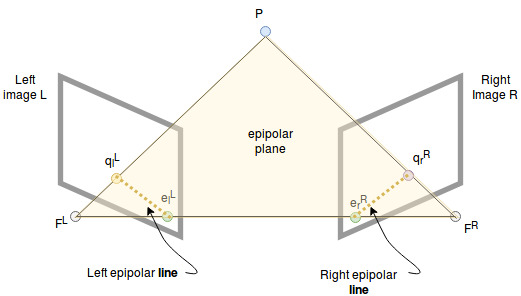
\includegraphics[width=0.7\linewidth]{epipolar.png}
\end{center}

\begin{intbox}
\textbf{The Epipolar Constraint (Why it matters):}
If you find a pixel in Image A, you don't need to search the \emph{entire} Image B to find its match (a 2D search). Geometry dictates that the match \emph{must} lie somewhere along a specific \textbf{epipolar line} in Image B (reducing it to a fast 1D search).
\end{intbox}

% ----------------------------------------------------------
\subsection{Essential and fundamental matrices (as needed)}
\begin{mathrule}
Relationship (calibrated intrinsics $K_1,K_2$):
\[
E = K_2^{\top} F K_1,
\qquad
F = K_2^{-\top} E K_1^{-1}.
\]
Use $F$ with \textbf{pixel} coordinates (physical image plane) and $E$ with \textbf{normalized} coordinates.
Also: one point $x$ in image 1 induces exactly \textbf{one} epipolar line $l_2 = F x$ in image 2.
\end{mathrule}

\subsubsection{Calibrated case: essential matrix ($\mat{E}$)}

\begin{mathrule}
\textbf{Epipolar constraint (calibrated / normalized coordinates):}\quad
\[
\tilde{\vct{x}}'^{\T}\,\mat{E}\,\tilde{\vct{x}} = 0,
\qquad \tilde{\vct{x}}\sim \mat{K}^{-1}\tilde{\vct{p}},\ \tilde{\vct{x}}'\sim \mat{K}'^{-1}\tilde{\vct{p}}'.
\]
\end{mathrule}

\begin{notebox}
In the calibrated case, $\mat{E}$ encodes the \textbf{relative pose} (up to scale) between the cameras.
\end{notebox}

\subsubsection{Uncalibrated case: fundamental matrix ($\mat{F}$)}

\begin{mathrule}
\textbf{Epipolar constraint (pixel coordinates):}\quad
\[
\tilde{\vct{p}}'^{\T}\,\mat{F}\,\tilde{\vct{p}} = 0.
\]
\end{mathrule}

\begin{defbox}
Given $\mat{F}$, the epipolar line in image 2 corresponding to point $\tilde{\vct{p}}$ in image 1 is:
\[
\mat{\ell}' = \mat{F}\,\tilde{\vct{p}}.
\]
Analogously, $\mat{\ell} = \mat{F}^{\T}\tilde{\vct{p}}'$ gives the line in image 1.
\end{defbox}

\subsubsection{Estimating $\mat{E}/\mat{F}$ from correspondences (high-level; \texorpdfstring{$\ge 8$}{>=8} point pairs)}

\begin{defbox}
\textbf{Estimation idea:} each correspondence yields one linear constraint on the entries of $\mat{F}$ (or $\mat{E}$).
Stack constraints from many correspondences and solve (least squares), typically with normalization and rank constraints.
\end{defbox}

\begin{itemize}
  \item Need at least 8 correspondences in the classic \textbf{8-point algorithm} (more is better).
  \item Use \textbf{RANSAC} to cope with outliers: repeatedly fit $\mat{F}/\mat{E}$ on minimal samples and keep the model with most inliers.
\end{itemize}

\begin{qbox}
\textbf{Exam pitfall:} without robust estimation, a few bad matches can completely break $\mat{F}/\mat{E}$ estimation.
\end{qbox}

% ----------------------------------------------------------
\subsection{Three-view geometry (trifocal tensor)}
\begin{notebox}
A trifocal tensor can be represented as a $3\times3\times3$ array with \textbf{27 coefficients} (it also satisfies internal constraints; its DOF is smaller than 27).
\end{notebox}

\subsection{Rectification and correspondence search}

\subsubsection{Image rectification (horizontal epipolar lines)}
\begin{notebox}
Epipolar lines are \emph{not} scanlines in general; \textbf{after rectification} they become (approximately) horizontal scanlines.
Rectification is done to make correspondence search \textbf{1D} (along rows) and typically \textbf{one-directional} (disparity).
\end{notebox}

\begin{defbox}
\textbf{Rectification} warps the two images so that corresponding epipolar lines become \textbf{horizontal scanlines}.
Then correspondence search becomes a 1D search along image rows.
\end{defbox}

\subsubsection{Scanline search and disparity}

\begin{defbox}
After rectification, a correspondence typically satisfies $y \approx y'$ and the remaining unknown is the horizontal shift.
\textbf{Disparity} is often defined as
\[
d = x_L - x_R
\]
(or the opposite sign depending on convention).
\end{defbox}

\begin{notebox}
Dense stereo estimates a disparity $d(x,y)$ for many/all pixels, producing a \textbf{disparity map}.
\end{notebox}

\subsubsection{Learning-based stereo (cost volumes; e.g., PSMNet idea)}
\begin{notebox}
A \textbf{cost volume} is built by combining left/right features across a range of disparities $d$ (e.g., concatenation or correlation),
yielding a volume of size roughly $H\times W\times D$.
A \textbf{3D CNN} then regularizes/aggregates matching costs across $(x,y,d)$ and regresses the final disparity.
\end{notebox}

\begin{notebox}
\textbf{Ordering constraint (rectified stereo):} along a scanline, the left-to-right order of corresponding points is preserved for opaque, non-occluded surfaces; it can be violated by \textbf{occlusions} and repeated structures.
\end{notebox}
% ----------------------------------------------------------
\subsection{Stereo depth reconstruction}

\subsubsection{Triangulation intuition (similar triangles)}

\begin{intbox}
Triangulation is ``ray intersection'':
back-project a pixel in each view to a 3D ray; the 3D point is where the rays meet (or come closest, with noise).
In the rectified stereo case, similar triangles give a simple depth--disparity relationship.
\end{intbox}

\subsubsection{Depth--disparity relationship}

\begin{mathrule}
\textbf{The Classic Stereo Formula:}
\[
\text{Depth } (Z) = \frac{\text{focal length } (f) \times \text{Baseline } (B)}{\text{disparity } (d)}
\]
\textbf{Crucial consequences for hardware design:}
\begin{itemize}
  \item \textbf{To see further/better (Sensitivity):} You need a larger Baseline $B$ (cameras further apart) or a larger focal length $f$ (zoom in). This spreads the disparity out over more pixels.
  \item \textbf{The far-distance problem:} For distant objects, $d$ approaches 0. Because $Z \propto 1/d$, a tiny 1-pixel error in matching (noise) will cause a massive error in the calculated 3D depth!
\end{itemize}
\end{mathrule}

\subsubsection{Dense disparity maps vs.\ sparse depth (overview)}

\begin{defbox}
\textbf{Sparse stereo:} compute depth only at matched keypoints (robust, low density).
\quad
\textbf{Dense stereo:} estimate depth for (almost) every pixel using matching costs + regularization/smoothness.
\end{defbox}

\begin{notebox}
Dense stereo struggles in textureless regions, repetitive patterns, and at occlusion boundaries (matching is ambiguous).
\end{notebox}

% ----------------------------------------------------------
\subsection{Affine / orthographic structure from motion (exam essentials)}
\begin{notebox}
\textbf{Affine shape:} reconstruction is only defined \textbf{up to an affine transformation} (not just scale).
A standard minimal statement used in class/exams: \textbf{2 views of 4 non-coplanar points} are sufficient to constrain affine shape (whereas 2 views of 3 points are not).
\end{notebox}

\begin{notebox}
\textbf{Affine camera counting (orthographic/affine model).}
A general affine camera can be written as a $2\times4$ matrix (8 parameters per view).
With $m$ views and $n$ points:
\[
\text{unknown coefficients} \approx 8m + 3n + 9,
\]
where the extra $+9$ reflects the inherent $3\times3$ affine ambiguity in factorization-based affine SfM.
\end{notebox}

\subsection{Structure from Motion (SfM)}

\subsubsection{Pipeline: match $\rightarrow$ estimate poses $\rightarrow$ triangulate}

\begin{defbox}
\textbf{SfM} generalizes stereo to \textbf{multiple} images: estimate \textbf{camera poses} and \textbf{3D points} jointly.
A typical pipeline:
\[
\text{detect/match features} \rightarrow \text{estimate relative motion} \rightarrow \text{triangulate} \rightarrow \text{refine}.
\]
\end{defbox}

\begin{itemize}
  \item Start from an initial image pair with good baseline.
  \item Incrementally add images: match to existing points, estimate new camera pose, triangulate new points.
  \item Refine by minimizing reprojection error (bundle adjustment; concept).
\end{itemize}

\begin{notebox}
\textbf{Exam Math: SfM Equation Counting ($m$ views, $n$ points)}
Each 3D point gives 2 equations (x, y pixel coordinates) per view. So we always have $\mathbf{2mn}$ equations.

\textbf{1. Raw Coefficient Counting (Simple):}
Camera = 12 unknowns, Point = 3 unknowns.
System is solvable if: $2mn \ge 12m + 3n$

\textbf{2. Projective DOF Counting (Advanced):}
Camera has 11 DOF, Point has 3 DOF, and the whole system has a 15-DOF coordinate system ambiguity.
System is solvable if: $2mn \ge 11m + 3n - 15$
\begin{itemize}
  \item \textbf{2 Views ($m=2$):} Needs $n > 7 \Rightarrow$ Minimum \textbf{8 correspondences}.
  \item \textbf{3 Views / 3 Points:} $18 \ge 27 \Rightarrow$ \textbf{False} (Not solvable).
\end{itemize}
\end{notebox}

\subsubsection{What SfM reconstructs (cameras + sparse 3D points; scale ambiguity)}

\begin{intbox}
SfM typically outputs:
\textbf{(i)} camera poses for each image and
\textbf{(ii)} a \textbf{sparse} 3D point cloud (from feature tracks).
Absolute \textbf{scale} is ambiguous without additional information (known baseline, IMU, GPS, etc.).
\end{intbox}

\begin{qbox}
\textbf{Exam pitfall:} multi-view geometry is powerful but fragile:
bad matches $\Rightarrow$ wrong $\mat{F}/\mat{E}$ $\Rightarrow$ wrong rectification/triangulation $\Rightarrow$ broken reconstruction.
Robust matching + calibration/undistortion are essential.
\end{qbox}

% ==========================================================
\section{3D Vision}

\begin{intbox}
So far we mostly interpreted images as \emph{2D} signals (classification, segmentation, detection) and then recovered
\emph{3D} structure from \emph{multiple views} (stereo, SfM). In \textbf{3D Vision} we focus on how depth/shape can be
\emph{represented}, \emph{predicted} (often learning-based), and \emph{rendered} (NeRF).
\end{intbox}

% ----------------------------------------------------------
\subsection{Depth from X (overview)}

\subsubsection{Depth from stereo / multiple views (recap)}
\begin{defbox}
\textbf{Depth from stereo / multiple views:} infer depth from \textbf{parallax} (viewpoint change).
Matching corresponding points constrains depth; larger baseline generally increases depth sensitivity.
\end{defbox}
\begin{itemize}
  \item \textbf{Stereo:} two calibrated views $\Rightarrow$ disparity $\Rightarrow$ depth (dense or sparse).
  \item \textbf{Multi-view / SfM:} many views $\Rightarrow$ estimate camera poses + sparse 3D points (then densify).
\end{itemize}
\begin{notebox}
This is the ``classical'' route: it relies on (i) feature extraction, (ii) matching, (iii) geometry, and (iv) calibration.
\end{notebox}

\subsubsection{Motivation for learning-based depth estimation}
\begin{intbox}
\textbf{Why learn depth?} Classical matching is brittle: pixel appearance depends on \emph{reflectance}, \emph{shape},
and \emph{shading}, but we only want shape. This makes correspondence (and thus depth) ill-posed in practice.
\end{intbox}

\begin{notebox}
\textbf{Depth from defocus (DfD) exam note.} Defocus cues require \textbf{texture/high-frequency content}; in \textbf{uniform regions} blur is ambiguous.
CNN features (including early/mid conv layers) can correlate with focus/blur primarily in \textbf{non-uniform (textured)} regions.
\end{notebox}

\begin{defbox}
\textbf{Depth from X:} depth estimation using cues other than multi-view parallax, e.g.\ \textbf{shading} or
\textbf{defocus} (focus blur). Each cue requires additional assumptions/models about image formation.
\end{defbox}

% ----------------------------------------------------------
\subsection{Depth maps}

\subsubsection{What a depth map represents (camera frame)}
\begin{defbox}
A \textbf{depth map} stores one scalar per pixel: the distance from the camera to the observed surface point along that pixel's viewing ray.
Together with RGB it forms an \textbf{RGB-D} image (often called ``2.5D'').
\end{defbox}

\begin{notebox}
Depth maps are view-dependent: they represent only what is visible from the camera (occlusions remove information).
Depth can be captured directly by some sensors (e.g., structured light / time-of-flight devices such as Microsoft Kinect).
\end{notebox}

\subsubsection{Structured light with Gray codes (exam essentials)}
\begin{notebox}
\textbf{Gray code property:} neighboring codewords differ by \textbf{Hamming distance 1} (only one bit changes), reducing decoding errors at boundaries.
For resolution $W\times H$, you need $\lceil\log_2 W\rceil$ patterns for columns and $\lceil\log_2 H\rceil$ for rows.
Example: $1024\times1024$ needs $10+10=\textbf{20}$ images (without additional inverse/complement patterns).
\end{notebox}

\subsubsection{Light transport and Helmholtz reciprocity (dual photography)}
\begin{notebox}
Model light transport as a linear map: camera image $c = T\,p$ (projector pattern $p$, transport matrix $T$).
\textbf{Helmholtz reciprocity} implies a swap of emitter/sensor corresponds to the \textbf{transpose} mapping ($T^\top$).
Thus \textbf{dual photography}: $p = T^\top c$.
If $c$ is \textbf{uniform white}, then $p$ visualizes the scene as seen from the \textbf{projector viewpoint} under uniform camera-side illumination.
\end{notebox}

\subsubsection{How to evaluate depth maps (common metrics, high-level)}
Two common viewpoints (as shown in the lecture):
\begin{itemize}
  \item \textbf{Per-pixel errors} between predicted and measured depth (after masking invalid pixels).
  \item \textbf{Log-depth errors} to reduce sensitivity to absolute scale and emphasize relative depth accuracy.
\end{itemize}

\begin{mathrule}
\textbf{Per-pixel loss on log-depth (lecture):}\quad
given ground truth $y_i$ and prediction $y_i^\ast$ at pixel $i$,
\[
D_{L2}(y,y^\ast) = \frac{1}{n}\sum_{i=1}^{n}\left(\log y_i - \log y_i^\ast\right)^2.
\]
(We estimate \emph{log depth} instead of depth.)
\end{mathrule}

\subsubsection{Scale-depth ambiguity (monocular depth)}
\begin{intbox}
\textbf{Monocular ambiguity:} a small close object can produce the same image as a large far object.
From a single image, \textbf{absolute scale} is fundamentally ambiguous without additional cues/priors.
\end{intbox}

\subsubsection{Scale-invariant error (idea and why it helps)}
\begin{mathrule}
\textbf{Scale-invariant loss (lecture):}\;
\[
D_{SI}(y,y^\ast)=\frac{1}{n}\sum_{i=1}^{n}\left(\log y_i - \log y_i^\ast + \alpha(y,y^\ast)\right)^2,
\qquad
\alpha(y,y^\ast)=\frac{1}{n}\sum_{j=1}^{n}\left(\log y_j - \log y_j^\ast\right).
\]
Intuition: $\alpha$ compensates a global scale offset in log-space (a global multiplicative depth scaling).
\end{mathrule}

\subsubsection{Predicting depth maps (high-level pipeline)}
\begin{defbox}
\textbf{Learning setup (monocular depth):}\;
train a CNN that maps an RGB image ($3\times H\times W$) to a depth map ($1\times H\times W$) using paired training data
(RGB, measured depth) and a per-pixel loss.
\end{defbox}

\begin{notebox}
Depth supervision can come from RGB-D sensors or from multi-view reconstruction pipelines.
\end{notebox}

% ----------------------------------------------------------
\subsection{Surface normals}

\subsubsection{Normals as local surface orientation}
\begin{defbox}
A \textbf{surface normal map} stores a 3D unit vector per pixel ($3\times H\times W$) describing the local surface orientation
(perpendicular to the tangent plane).
\end{defbox}

\begin{notebox}
Depth and normals are tightly related:
\begin{itemize}
  \item depth $\rightarrow$ normals via spatial derivatives (gradients of depth / reconstructed surface),
  \item normals $\rightarrow$ depth via integration (a PDE / reconstruction problem).
\end{itemize}
\end{notebox}

\subsubsection{Predicting and evaluating normals (angular error intuition)}
\begin{defbox}
Normals are evaluated by \textbf{angular error}:
two unit normals agree if their angle is small (0° is perfect).
\end{defbox}

\begin{mathrule}
\textbf{Cosine similarity / angle:}\quad
\[
\vct{n}\cdot \vct{n}^\ast = \|\vct{n}\|\;\|\vct{n}^\ast\|\cos\theta
\quad\Rightarrow\quad
\theta = \arccos\!\left(\frac{\vct{n}\cdot \vct{n}^\ast}{\|\vct{n}\|\;\|\vct{n}^\ast\|}\right).
\]
A common loss uses the dot product (cosine similarity) per pixel.
\end{mathrule}

% ----------------------------------------------------------
\subsection{3D shape representations}

\subsubsection{Voxel grids (occupancy in a 3D grid; pros/cons)}
\begin{defbox}
\textbf{Voxel grid:} discretize 3D space into a $V\times V\times V$ grid; each voxel stores occupancy (or related properties).
Conceptually ``segmentation in 3D''.
\end{defbox}
\begin{itemize}
  \item (+) Simple, regular structure; can use 3D CNNs.
  \item (-) Memory scales as $O(V^3)$ $\Rightarrow$ high resolution is expensive; fine details require very large $V$.
\end{itemize}
\begin{notebox}
Example learning pipeline (as shown): 2D CNN features $\rightarrow$ 3D CNN $\rightarrow$ voxel occupancy;
trained with per-voxel cross-entropy loss.
\end{notebox}

\subsubsection{Point clouds (set of 3D points; pros/cons)}
\begin{defbox}
\textbf{Point cloud:} represent a shape as a set of $P$ 3D points (typically on the surface).
\end{defbox}
\begin{itemize}
  \item (+) Efficient for fine structures without a dense 3D grid.
  \item (-) Unordered set $\Rightarrow$ needs special architectures/losses; no explicit connectivity/surface.
  \item (-) Rendering or surface extraction often needs post-processing (e.g., meshing).
\end{itemize}

\subsubsection{ICP (Iterative Closest Point) complexity (exam essentials)}
\begin{notebox}
ICP alternates between nearest-neighbor matching and estimating a rigid transform.
Naive correspondence search is $O(N^2)$; with a k-d tree (or similar spatial index) it is roughly $O(N\log N)$ per iteration.
\end{notebox}

\subsubsection{Meshes (vertices + faces; graphics standard; pros/cons)}
\begin{defbox}
\textbf{Mesh:} vertices + faces (usually triangles). Standard representation in graphics; explicitly encodes surface connectivity.
\end{defbox}
\begin{itemize}
  \item (+) Adaptive: allocate more triangles where detail is high.
  \item (+) Can attach/interpolate attributes (RGB, texture coordinates, normals, \dots).
  \item (-) Learning/optimization is harder than voxels due to topology/connectivity constraints.
\end{itemize}

\subsubsection{Implicit surfaces (inside/outside function; link to rendering)}
\begin{defbox}
\textbf{Implicit surface:} represent geometry via a function $f(x,y,z)$ (e.g., occupancy / inside-outside / density),
rather than an explicit list of points or voxels. This viewpoint connects naturally to rendering and NeRF-style methods.
\end{defbox}

% ----------------------------------------------------------
\subsection{Neural Radiance Fields (NeRF)}

\subsubsection{Recap: pinhole cameras and rays (origin + direction)}
\begin{defbox}
A pixel corresponds to a \textbf{camera ray}
\[
\vct{r}(t)=\vct{o}+t\,\vct{d},
\]
with ray origin $\vct{o}$ at the camera center and direction $\vct{d}$ through the pixel (after applying intrinsics/extrinsics).
\end{defbox}

\subsubsection{Volume rendering (intuition)}

\begin{mathrule}
\textbf{Volume Rendering Equation (How to calculate pixel color):}
We shoot a ray through the 3D scene. The final color $C$ of the pixel is the sum (integral) of all light emitted along that ray, \emph{minus} the light that gets blocked before reaching the camera.
\[
C(\text{ray}) = \int_{\text{near}}^{\text{far}} \underbrace{T(t)}_{\text{Transmittance}} \times \underbrace{\sigma(t)}_{\text{Density}} \times \underbrace{c(t)}_{\text{Color}} \,dt
\]
\begin{itemize}
  \item \textbf{Color ($c$):} The color emitted by a specific 3D point.
  \item \textbf{Density ($\sigma$):} How solid/opaque is the point? (Does it emit/block light at all?)
  \item \textbf{Transmittance ($T$):} The probability that the light from this point actually reaches the camera without hitting a solid object ($\sigma$) in front of it first.
\end{itemize}
\end{mathrule}

\subsubsection{NeRF parameterization (density + color along rays)}
\begin{defbox}
\textbf{NeRF:} train a neural network (typically an MLP) that maps
position $\vct{p}=(x,y,z)$ and viewing direction $\vct{d}=(\theta,\phi)$ to
\[
(\sigma(\vct{p}),\ \vct{c}(\vct{p},\vct{d})).
\]
Rendering an image is then differentiable volume rendering along camera rays.
\end{defbox}

\begin{notebox}
\textbf{Binary opacity thought experiment (exam-style).} If $\sigma$ (opacity/density) were forced to be \textbf{binary} (0/1),
the model can still represent \textbf{opaque surfaces} (diffuse + view-dependent/specular appearance),
but it cannot represent \textbf{transmission/refraction} or semi-transparent volumetric effects.
\end{notebox}

\subsubsection{Training setup and key limitations (scene-specific, compute)}
\begin{itemize}
  \item \textbf{Training signal:} given multiple \textbf{posed images} (known camera intrinsics/extrinsics), sample rays and minimize an image reconstruction loss
        between rendered pixel colors and observed pixel colors (often simple $L_2$).
  \item \textbf{Scene-specific:} classical NeRFs are typically trained per scene (no universal pretraining by default).
  \item \textbf{Compute:} training and rendering are expensive due to many samples along many rays (practical accelerations exist).
  \item \textbf{Limitations:} dynamic scenes, strong view-dependent effects, and occlusions/thin structures can be challenging without extensions.
\end{itemize}

\begin{notebox}
NeRF is primarily about \textbf{novel view synthesis} (rendering from new viewpoints), but it also induces a rich
3D scene representation (density field) that can be queried for geometry and depth cues.
\end{notebox}

\end{document}